%%%%%%%%%%%%%%%%%%%%%%%%%%%%%%%%%%%%%%%%%%%%%%%%%%%%%%%%%%%%%%%%%%%
%                                                                 %
%                            CHAPTER TWO                          %
%                                                                 %
%%%%%%%%%%%%%%%%%%%%%%%%%%%%%%%%%%%%%%%%%%%%%%%%%%%%%%%%%%%%%%%%%%%

\chapter{COLLECTION} \label{sec:collection}

\begin{figure*}[t]%
    \centering
    \subfloat {{ $\vcenter{\hbox{ \includegraphics[width=0.75\textwidth]{resources/printout.jpg} }}$ }}%
    \caption[Example Printout Returned to Each Citizen Scientist]{\textbf{Example Printout Returned to Each Citizen Scientist.}  Each participating citizen scientist recieved a printout showing a map of where the car drove (in blue) and information for three animals seen by that photographer (black, red, and green).  The other sightings for the three animals were also marked on the map.  This was the printout that was given to citizen scientist ``A'' in car ``8 WHITE''.  This participant saw one new animal (red) and resighted two animals (black and green).  The pictures taken by the participant are shown on the left and the matching animal (or information on the new sighting) is shown on the right.  The recognition matches were provided by IBEIS using an initial database.}
        \label{fig:printout}
\end{figure*}

Every citizen scientist who volunteered for the GZGC was first registered and then sent out into the NNP to collect image data.  After they completed their collection, all participants returned to the registration site so that their collected image data could be contributed, and subsets could be processed on-site.  The processing software used during the GZGC was developed as a client-server model (connected using a local, offline network); import client machines copied the image data    camera memory cards and then submitted them to a central server for processing.  Each participating citizen scientist received a printout showing a brief, preliminary analysis of the images they took.  An example printout can be seen in Figure \ref{fig:printout}.  The volume of collected data was too large relative to the processing capabilities of the system for more detailed feedback the day of collection.  All of the import client machines and the central processing server were laptop computers and needed to work without Internet connectivity to process the images.  The central IBEIS server laptop was a 64-bit AMD quad-core Lenovo laptop with 16 GB of RAM running Ubuntu 14.04.  The on-site data collection steps are described in more detail in the remainder of this chapter and are summarized in Figure \ref{fig:process}.

%Given this workflow, the GZGC operated under the following constraints and assumptions:
%\begin{enumerate}
%   \item The automatic or manual processing of the collected data was computationally intensive,
%   \item The collection protocol training for the citizen scientist needed to be minimal and be taught in a short period of time (5-15 minutes),
%   \item A small, uniform random sampling of the data collected by the citizen scientist was sufficient to summarize their entire data as a whole,
%   \item A participating citizen scientist was required to bring their own transportation and a personal camera with a removable memory card,
%   \item A participating citizen scientist expected some level of immediate feedback from the data they had collected that day, and
%   \item The processing of the collected data had to be agnostic to input order.
%\end{enumerate}

%For the GZGC,IBEIS producing the computer vision analytics was constrained by the efficiency of algorithms and the computational power of the server laptop;  on average, IBEIS could process an image, on average, in a few seconds.  Due to this processing bottleneck, immediate on-site processing of \textit{all} images collected by a citizen scientist was computationally infeasible; the semi-automatic results of detection and identification had to be manually reviewed.  This review process was ultimately a limiting man-power bottleneck that could have severely impacted the responsiveness of the GZGC if we had processed all images collected by a citizen scientist immediately and on-site.

%This chapter describes how image data was gathered and saved from the citizen scientist, sampled a small set of images for processing, processed the small image set by IBEIS, and then generated a printout result for the citizen scientist to keep.  It should be explicitly mentioned that the printout is critical to the success of the overall data collection;  the printout provides each citizen scientist with a reason to continue participate in future data collections as it is tangible proof of their contributions being utilized for some scientific goal, but also unctions as a potential marketing flier to facilitate the recruitment of future citizen scientists.  The time from when the citizen scientist returned with collected image data to when the printout was generated was 2 to 5 minutes, depending on the number of images collected by that citizen scientist and the processing load on the server at the time that individual returned.  An overview of the collection process can be viewed in Figure \ref{fig:process}.

\begin{figure*}[t]%
    \centering
    \subfloat {{ $\vcenter{\hbox{ 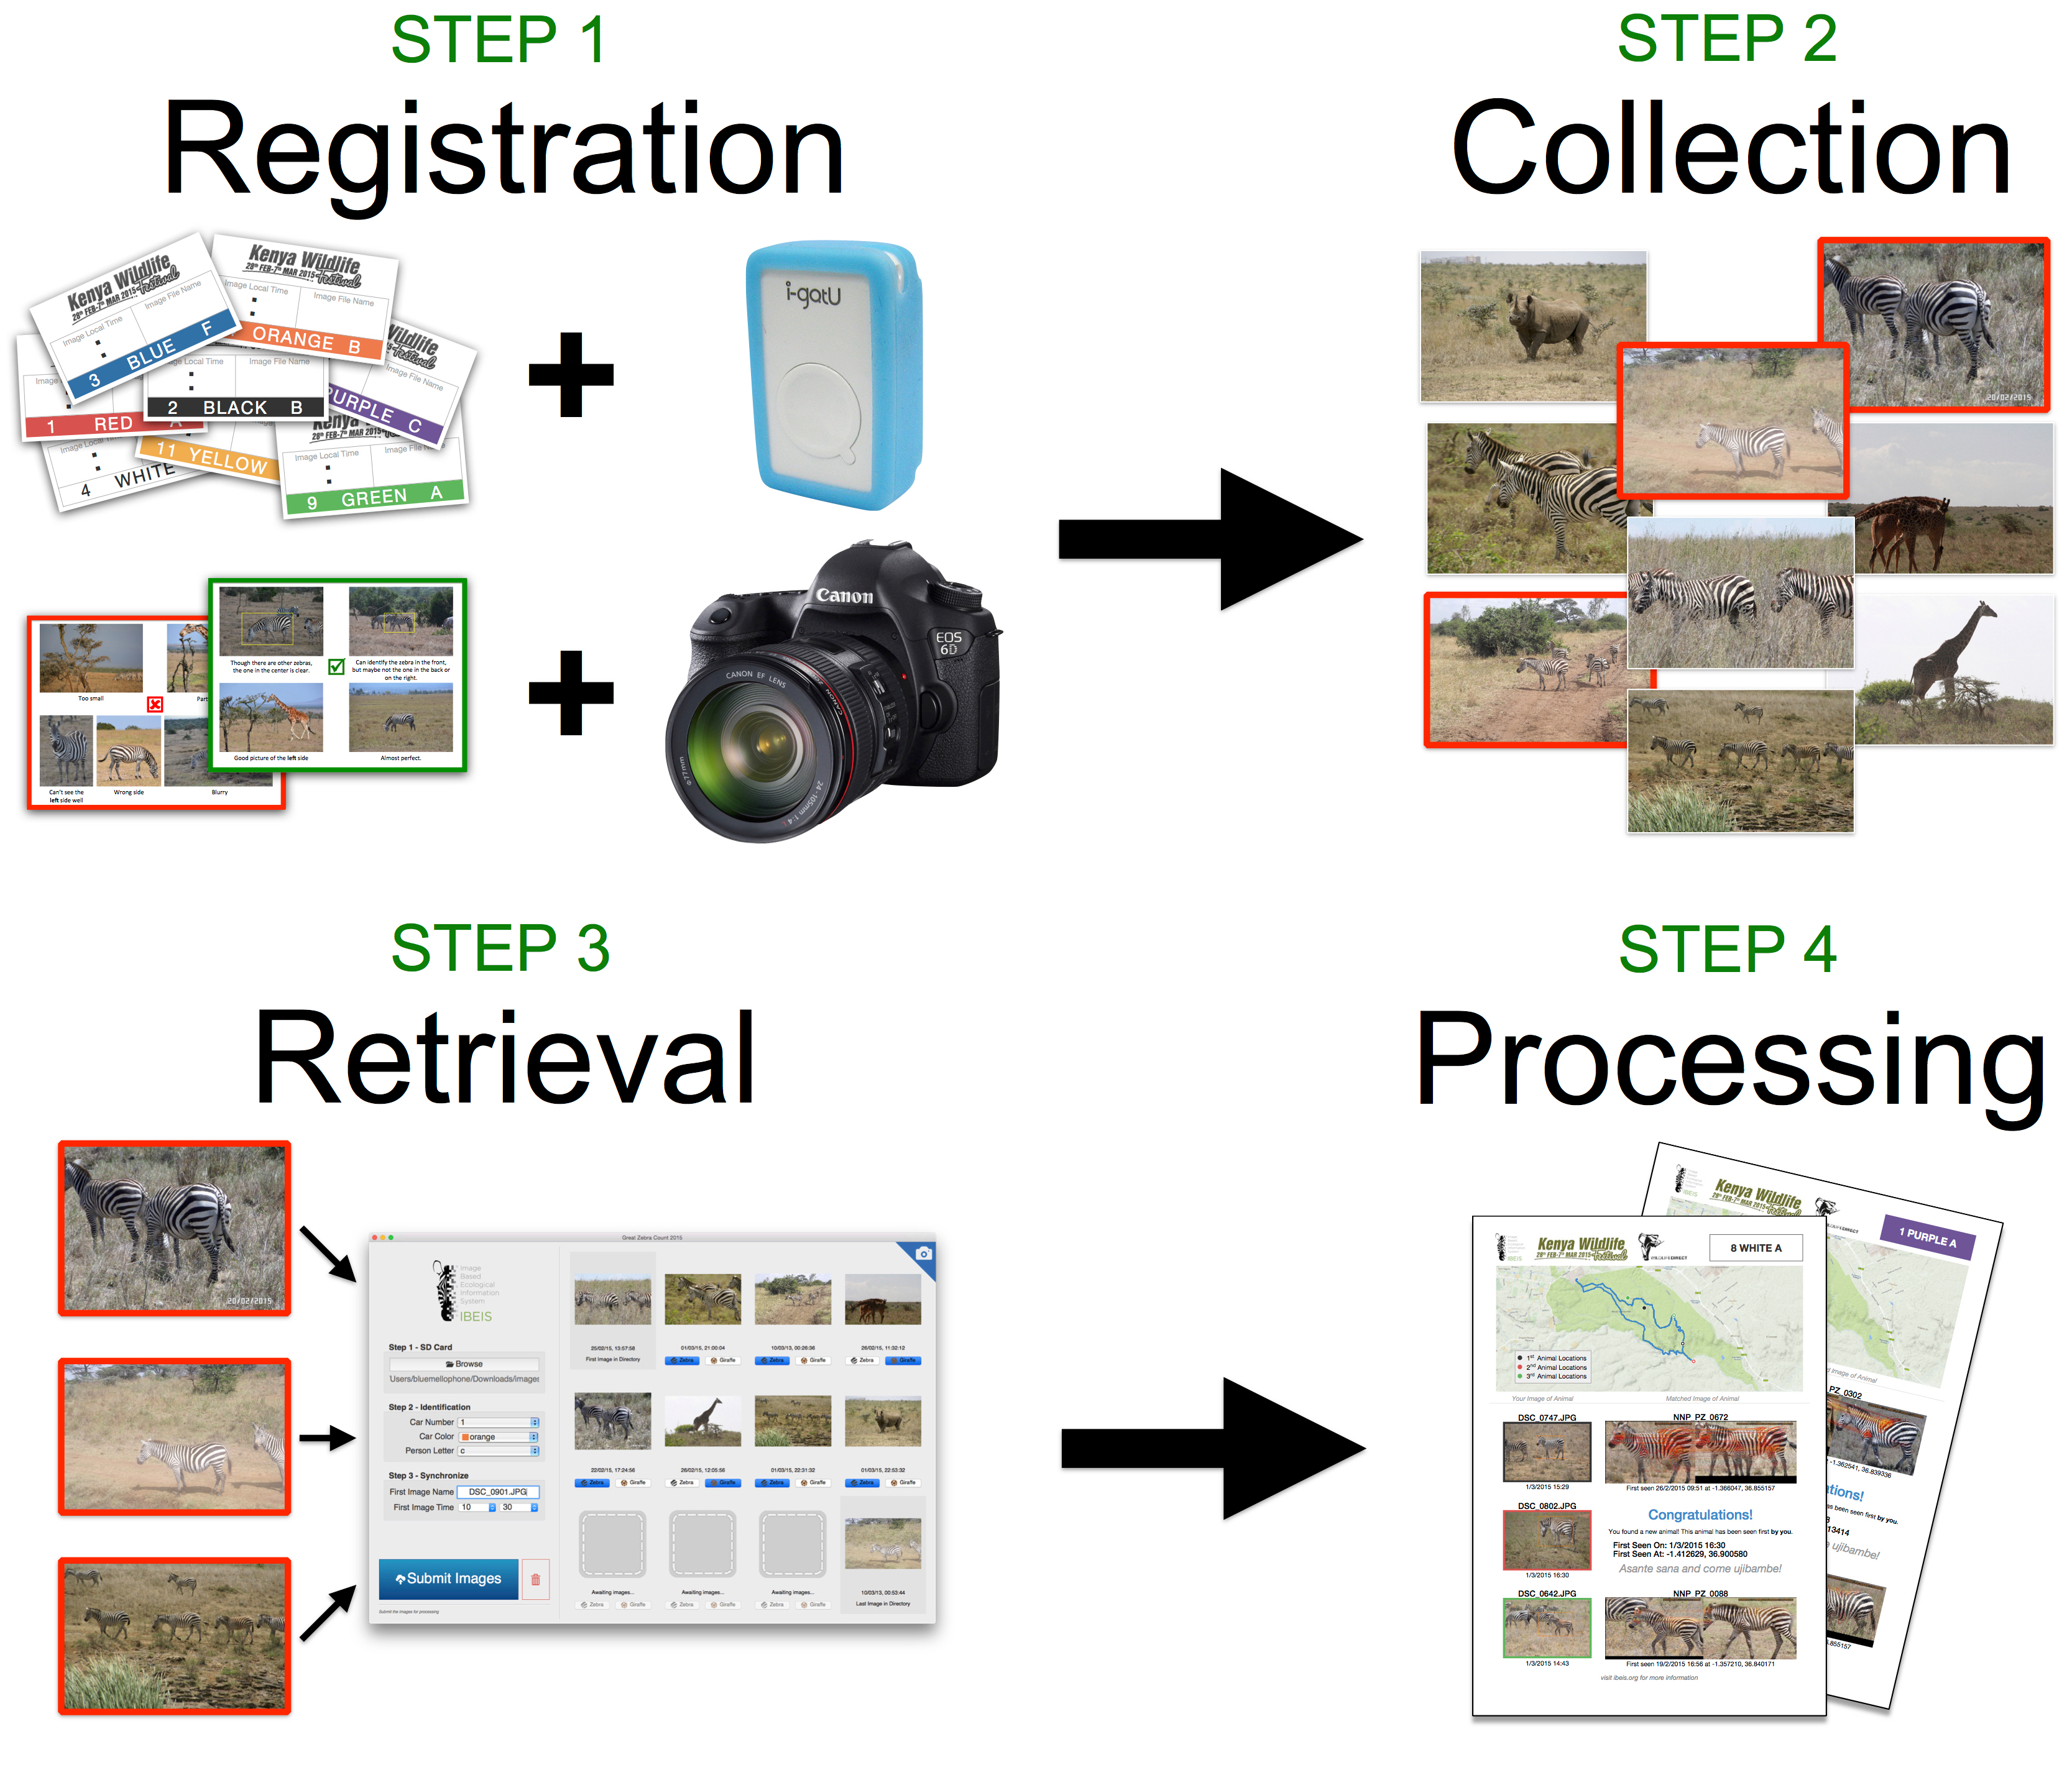
\includegraphics[width=0.90\textwidth]{resources/process_square_spaced.jpg} }}$ }}%
    \caption[Data Collection Proceedure during \textit{The Great Zebra \& Giraffe Count}]{\textbf{Data Collection Proceedure during \textit{The Great Zebra \& Giraffe Count}.}  Step 1 (Registration): citizen scientists with cameras were registered by being given a registration card, a GPS dongle (for the car), and a training sheet.  Step 2 (Collection): participants were instructed to go into the NNP and take pictures of animals for specific species and viewpoints.  Step 3 (Retieval): all images were collected from the camera of returned citizen scientists along with metadata from the registration cards and GPS dongles; a subset (in red) of the collected images were sent to IBEIS for processing.  Step 4 (Processing): the results from IBEIS were recorded into a database and tabulated onto a printout, which was given to the participant to keep as a reward for their contributions.}
        \label{fig:process}
\end{figure*}

\section{Registration}
In order to contribute images to the GZGC, each participating citizen scientist had to be given a mechanism to synchronize \textit{when} and \textit{where} their images were taken.  In order to achieve this, we trained a team of IBEIS volunteers to coordinate registration and guide participants through a time and GPS registration.  Our procedure relied on citizen scientists bringing their own personal cameras because we did not have any to lend out.  This compounded the synchronization problem as our procedure had to function across a multitude of camera manufacturers and a range of photographer experience.  In order to eliminate the complexity and inefficiencies of registration, we opted to implement a process that was agnostic to camera manufacturer, language, and specific settings and precluded the need to investigate the potential intricacies of every camera.  A team of two IBEIS volunteers guided each participant through the following registration process:

\begin{enumerate}
    \item Each photographer was given a registration card with a unique, pre-selected, identification code defined by car number, car color, and person letter. The car numbers were in the range $[0-25]$; eight colors were used (red, orange, yellow, green, blue, purple, black and white) for the car color; the person letters were in the range $[A-F]$.  Each participating car was given a number and a color combination and each person in that car was given one of the letters, for a maximum of 6 people per car. If a car had more than 6 participants (e.g.\ in the event of a school bus), additional car number and color combinations were used until there were enough registration cards to assign to each participant.  The registration card's purpose was two fold: to standardize the data collection procedure and to eventually become a memento and marketing keepsake for the participant.  The back of the registration card also had contact information for the IBEIS team and information about the software.  An example registration card for participant ``A'' in the car ``1 RED'' can be seen in Figure \ref{fig:card}.
    \item For each participant, the current, local time of registration was written on the card.
    \item Using the participant's camera, an image was taken of the participant's registration card with the then-current time.  This image -- let's call it $Image_0$ -- was required to have been taken relatively close to when the local time was written on the card (within 30 seconds), because it was used to time synchronize all images taken by that camera upon return.
    \item Once $Image_0$ had been taken, the camera's digital display was used to record the file name (or sequence number) of $Image_0$ on the registration card.  At that point, the participant was registered with the GZGC and instructed to put away and save the registration card until after data collection.
    \item Finally, each car was given an i-gotU brand GPS dongle \footnote{www.i-gotu.com/product/USB\_GPS.html [Accessed: Nov. 1, 2015]}.   The GPS dongle made a new record every second (assuming acquired satellite signal) containing the UTC timestamp, the latitude position, the longitude position, the elevation, and other metadata.  The GPS records were used to localize all of the images taken by the cameras of all participants in that car.  In the rare event that the camera provided in-camera GPS EXIF data, it was discarded and replaced by the GPS dongle's GPS record, for consistency.
\end{enumerate}
The importance of $Image_0$ cannot be overstated: it functioned as a beginning bookend for what images belonged to the GZGC and also provided a digital backup copy of the physical registration card in the event it was lost or destroyed.  Citizen scientists in the GZGC were not required to clear their camera memory cards (although encouraged) in order to participate.  During the GZGC, a citizen scientist participating with a non-empty camera memory card was the overwhelmingly dominant scenario, even though marketing material for the GZGC encouraged participants to come with a clean memory card.  For those participants, $Image_0$ was used to mark the end of potentially sensitive images, which should have not been copied from the memory card.

\begin{figure}[t]%
%\begin{figure}[!htb]%
    \centering
    \subfloat {{ $\vcenter{\hbox{ \includegraphics[width=0.45\textwidth]{resources/card-front.jpg} }}$ }}%
    \subfloat {{ $\vcenter{\hbox{ \includegraphics[width=0.45\textwidth]{resources/card-back.jpg} }}$ }}%
        \caption[The Registration Card Given to Volunteer Citizen Scientists]{\textbf{The Registration Card Given to Volunteer Citizen Scientists.}  This figure shows the front (left) and back (right) faces of an example registration card.  Each participant recieved a card with a unique identification code.  This specific card was for car ``1 RED'' and for participant ``A'' within that vehicle.  The left box of the registration card was meant to hold the time of registration and the right box to hold the image filename or sequence number of $Image_0$.}
        \label{fig:card}
\end{figure}

\section{Collection}
Once a participant was registered, they were given brief training on \textit{how} and \textit{where} to take pictures.  The assigned zones and their respective coverages of the NNP can be seen in Figure \ref{fig:coverage} in Chapter \ref{sec:results}. The training was designed to ensure sufficient image quality and to provide park coverage.  Figure \ref{fig:images} shows example images that were collected by the citizen scientists during the GZGC.

Citizen scientists were instructed to only take pictures of certain species (e.g.\  zebra) and of consistent viewpoints (e.g.\ left-side).  We did not have to teach the differences between sub-species of zebra or giraffes considering the NNP only had the one sub-species of each, plains zebra (\textit{Equus quagga}) and Masai giraffe (\textit{Giraffa camelopardalis tippelskirchi}).  The viewpoint constraint resolves a symmetry ambiguity, which is caused by zebras (and giraffes) not being left-right symmetric (i.e.\ the left-side appearance is different from the right-side).  Therefore, due to this lack of symmetry, we cannot reliably know if we have seen an individual before if we only saw opposite sides.  Lastly, the participants were asked to avoid taking obstructed, poorly illuminated, or out-of-focus pictures or where the zebra was too distant to get a detailed picture.

To ensure park coverage, each participating car was assigned a zone within the NNP to take pictures.  Participants were instructed to start taking pictures only from inside their assigned zone, but they could continue to take pictures outside of their zone as they returned back to the registration site.  This constraint was to ensure adequate coverage of the assigned zone by attempting to reduce ``species fatigue'' -- the phenomenon where a photographer tires of taking pictures of a common species -- since it produces a sampling bias in the locations of animal sightings.  This bias can be tolerated outside of a participant's assigned zone, but should be discouraged in order to achieve a higher likelihood of capturing unbiased animal sightings in all zones.

\begin{figure*}[t]%
    \centering
    \subfloat {{ $\vcenter{\hbox{ 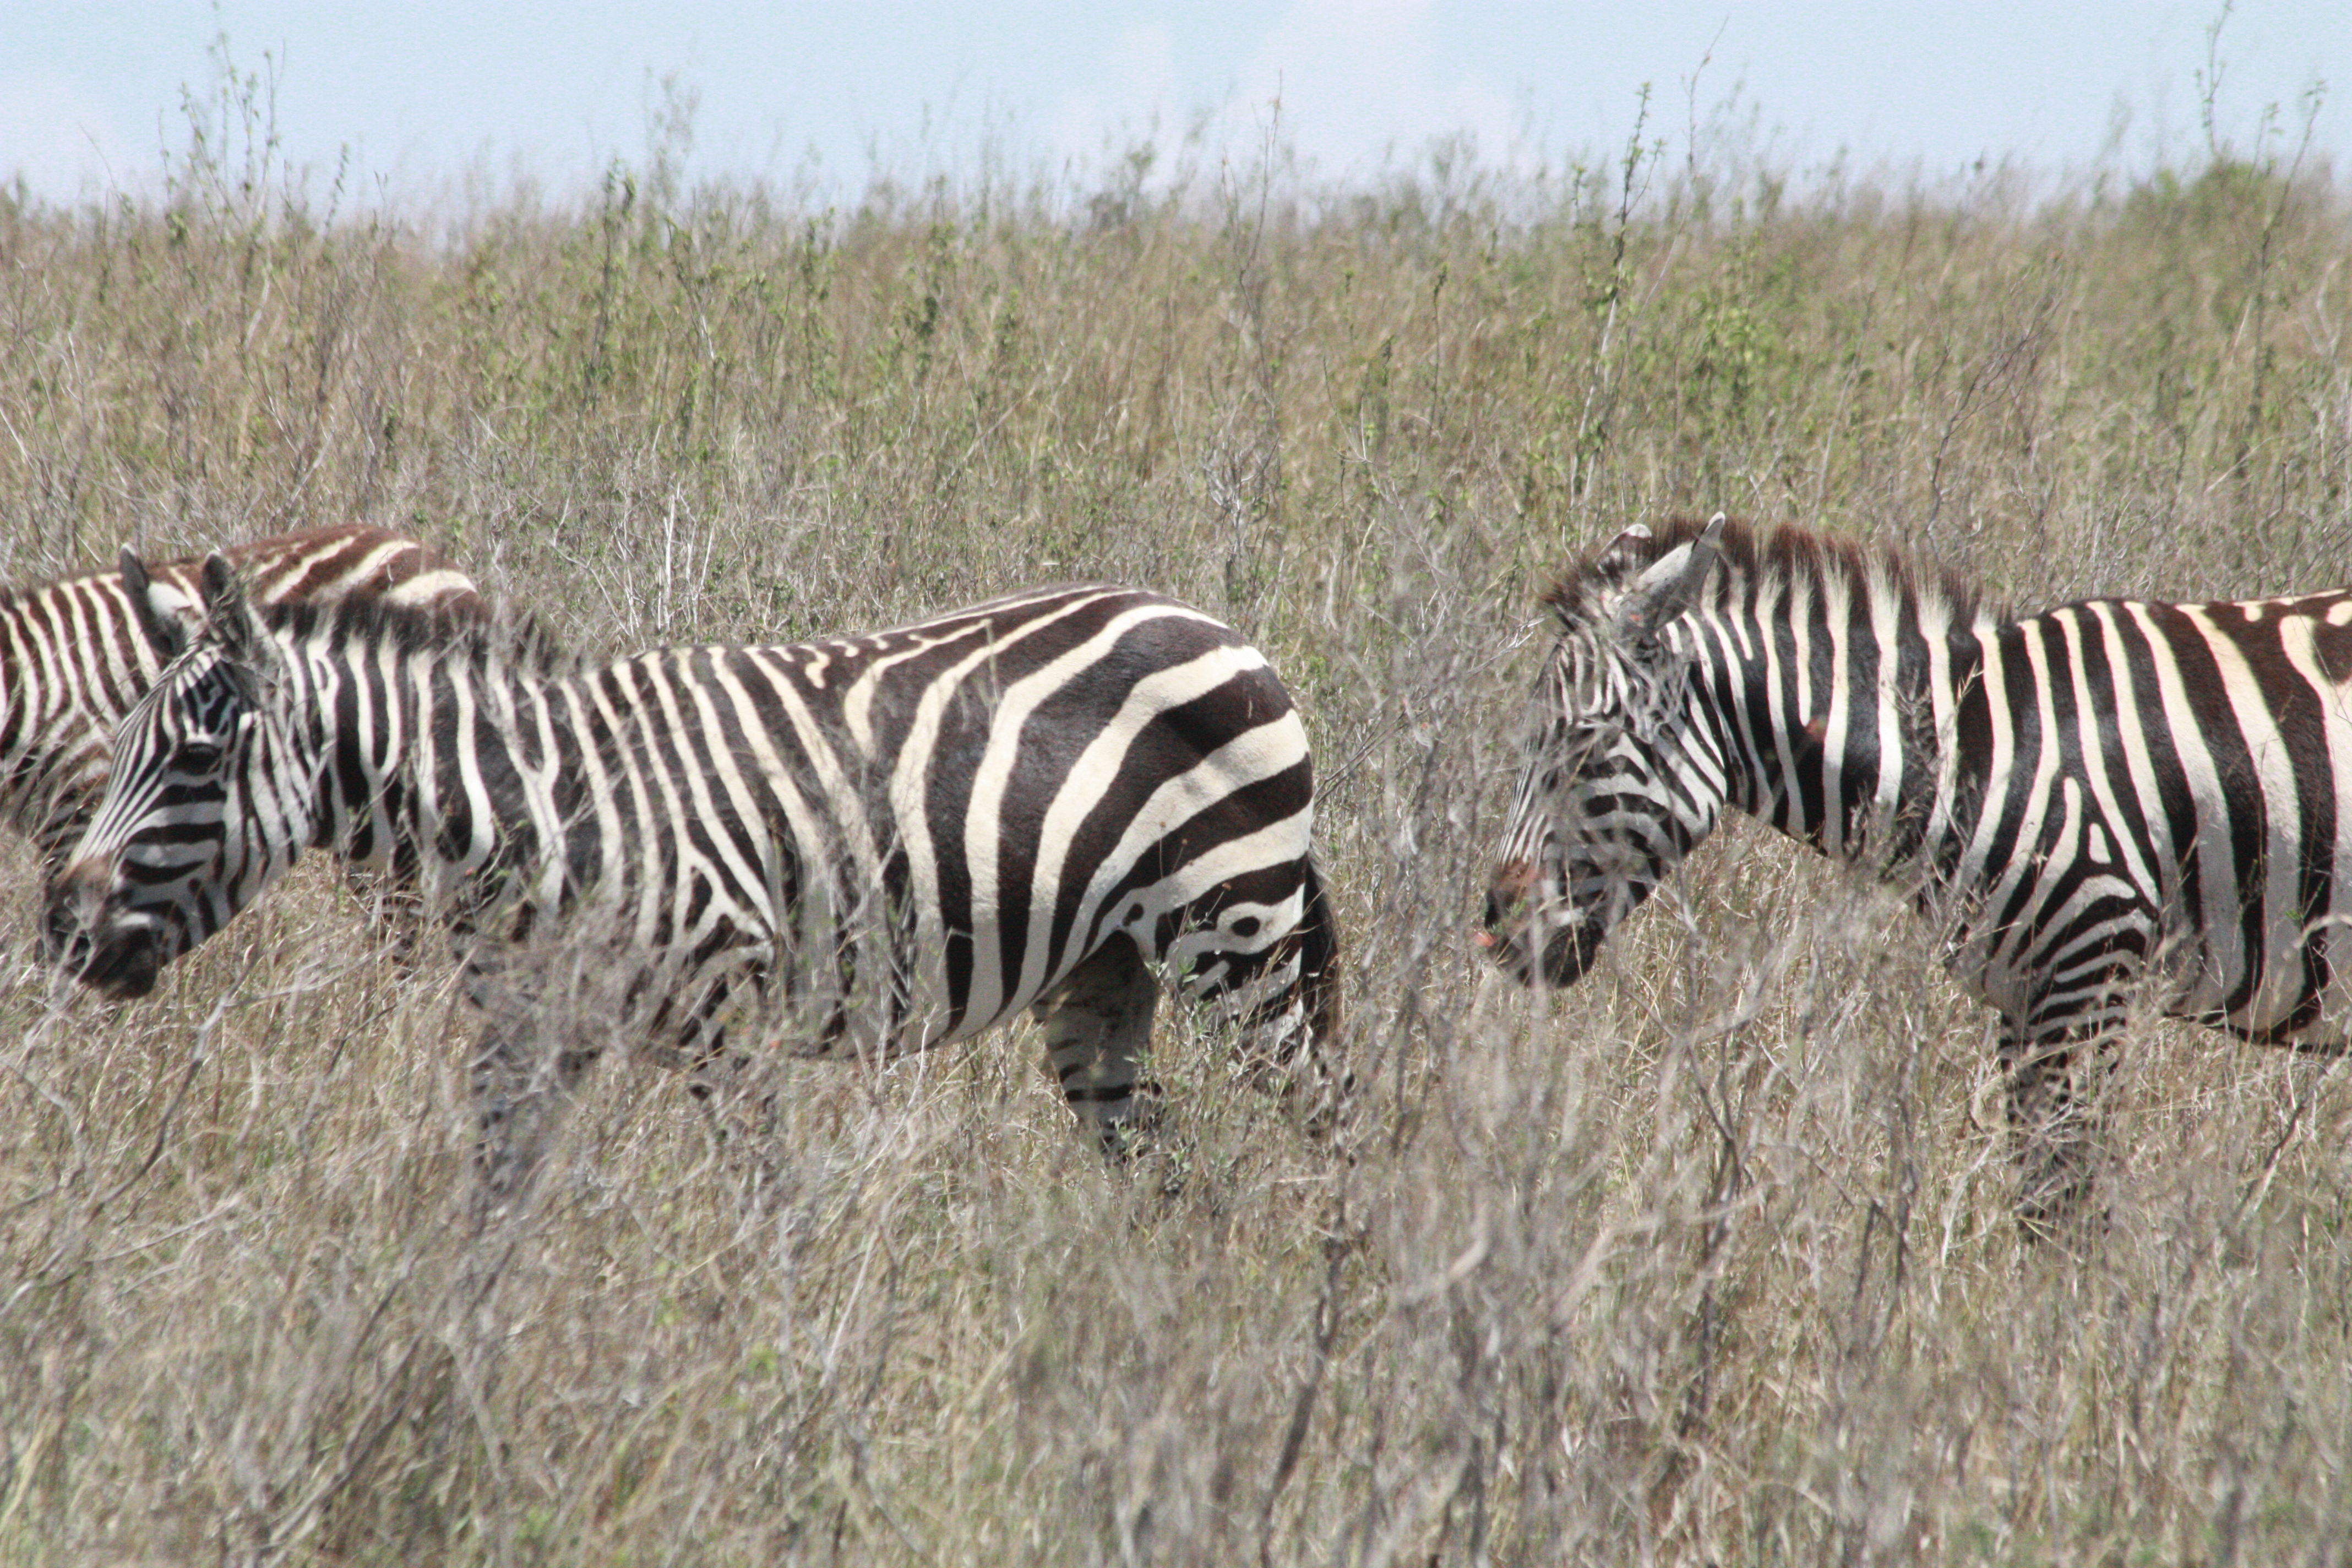
\includegraphics[width=0.16\textwidth]{resources/images/0b236c57-5023-e3e1-8c5d-c5a55d346ea8.jpg} }}$ }}%
    \subfloat {{ $\vcenter{\hbox{ \includegraphics[width=0.16\textwidth]{resources/images/0b456b34-dc14-3d3f-3dfa-833a3a31c8d1.jpg} }}$ }}%
    \subfloat {{ $\vcenter{\hbox{ 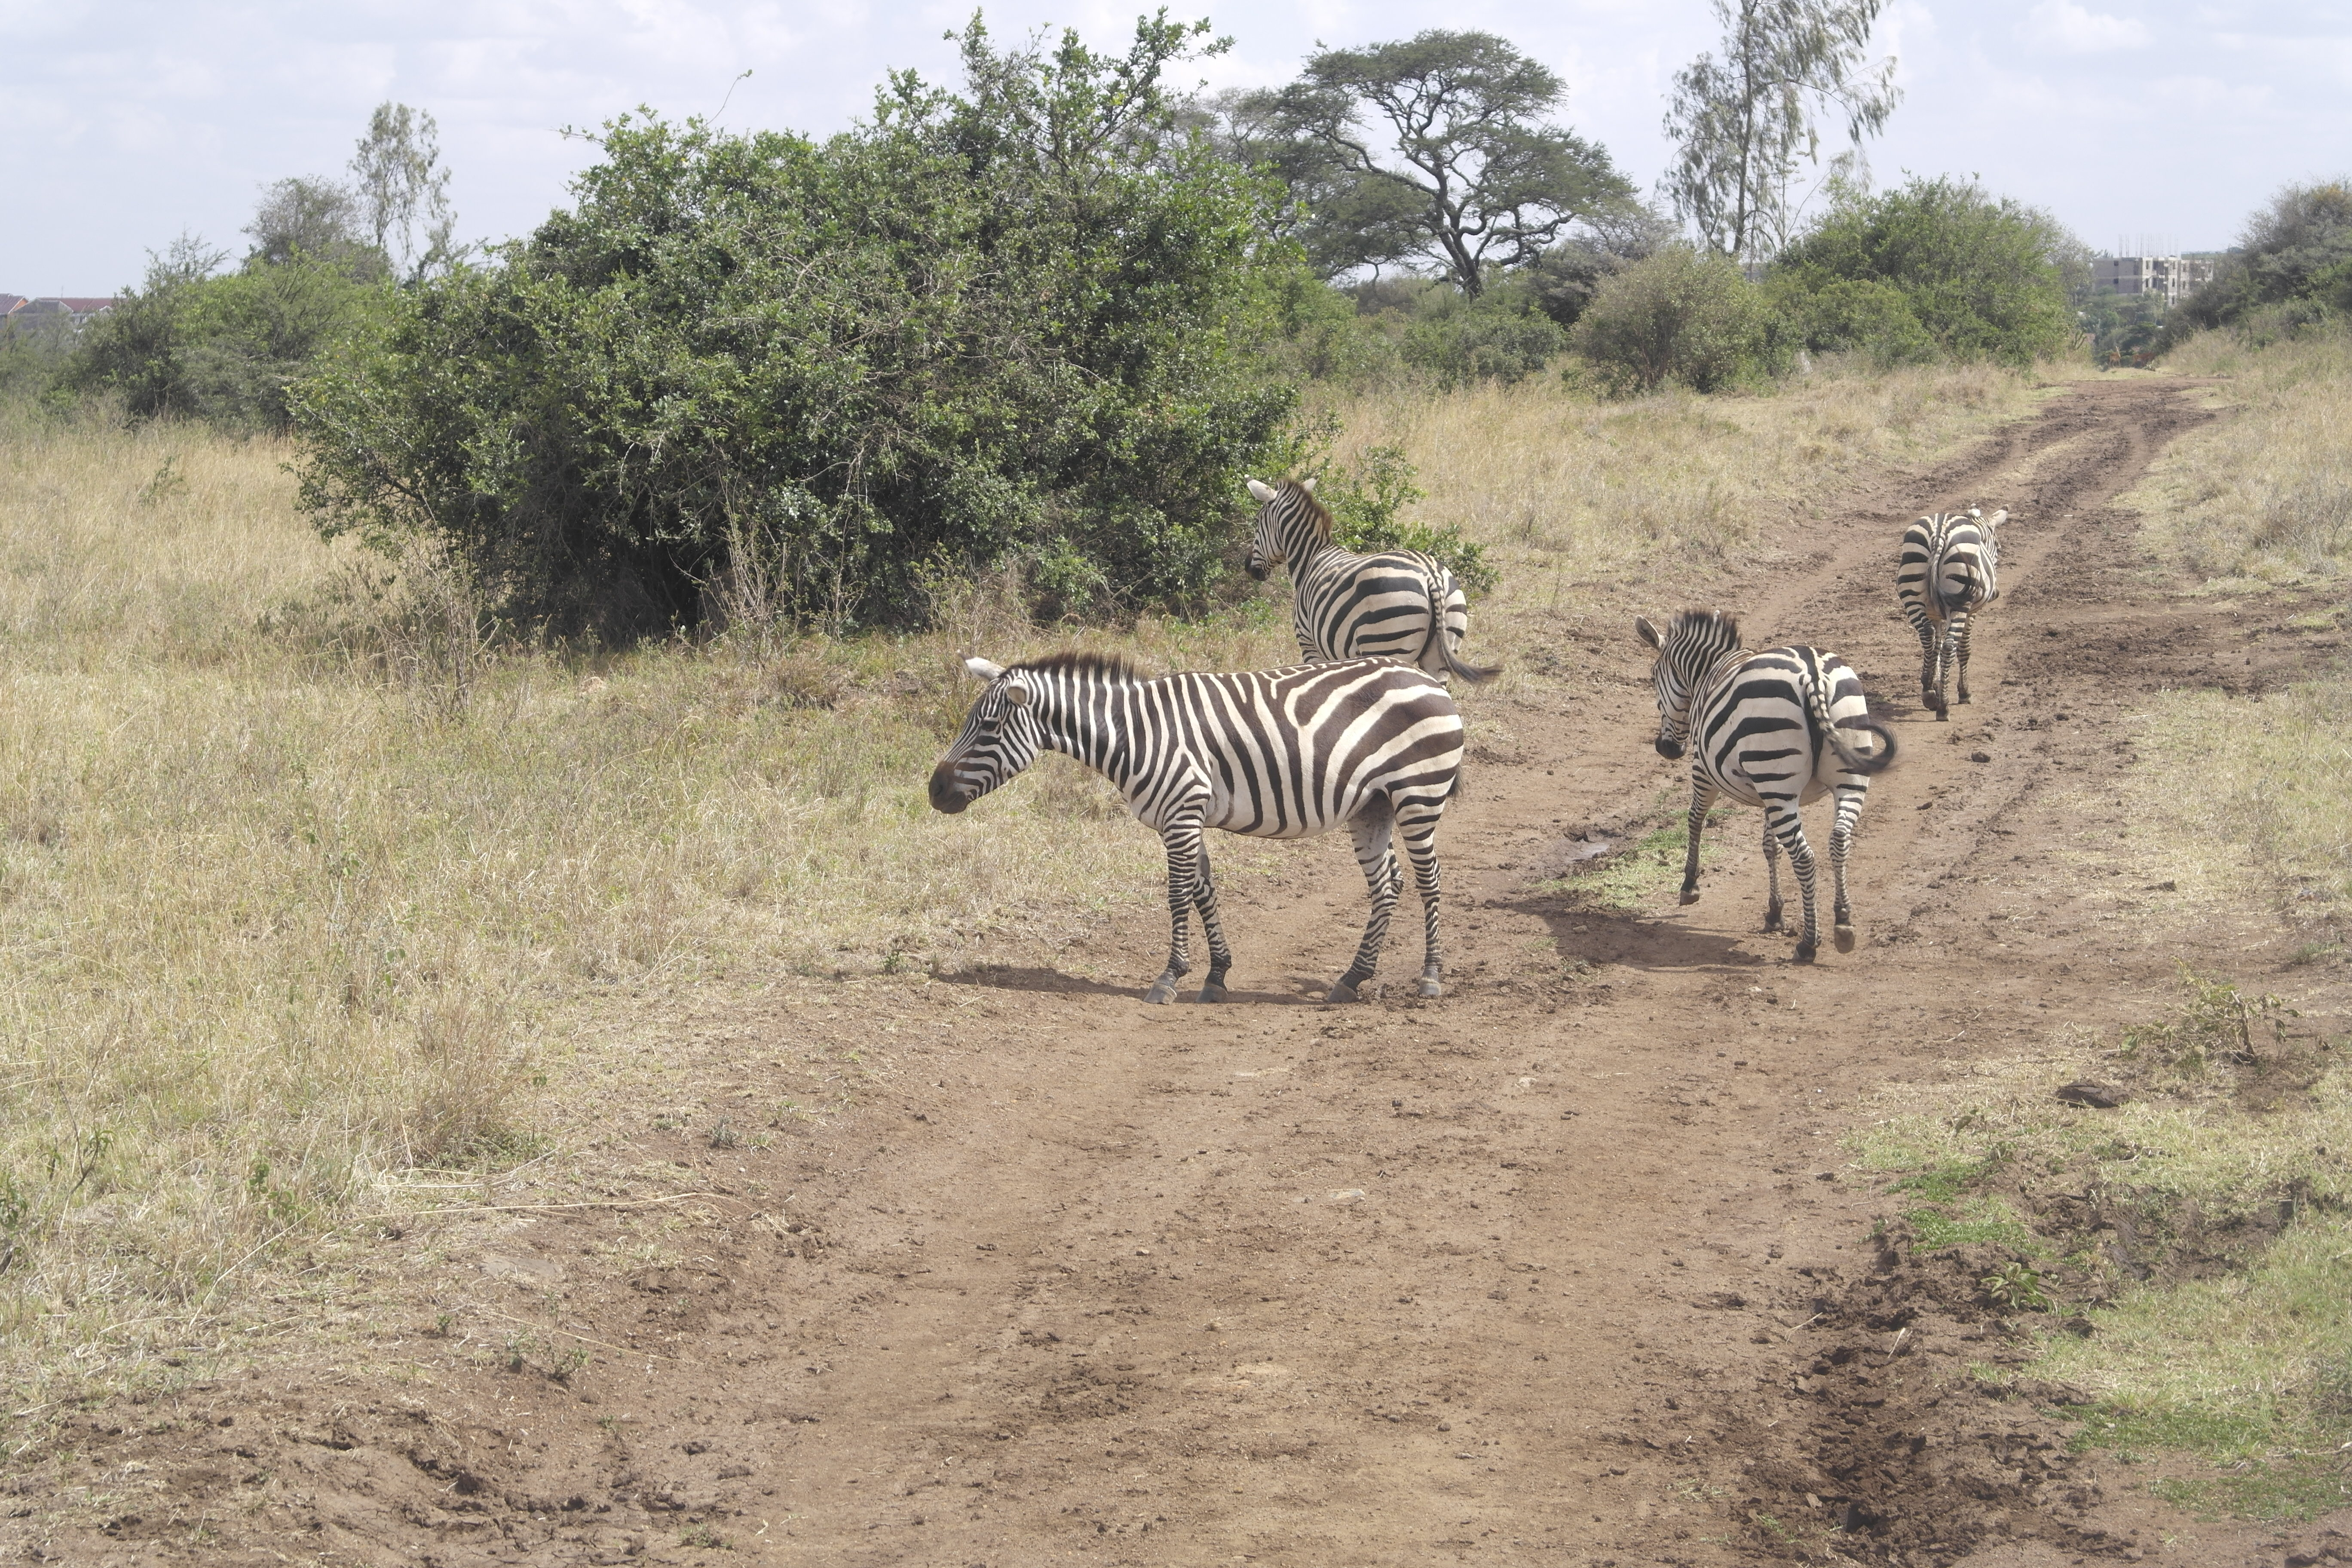
\includegraphics[width=0.16\textwidth]{resources/images/0b6993d5-ee88-04b3-0953-8a508857da42.jpg} }}$ }}%
    \subfloat {{ $\vcenter{\hbox{ 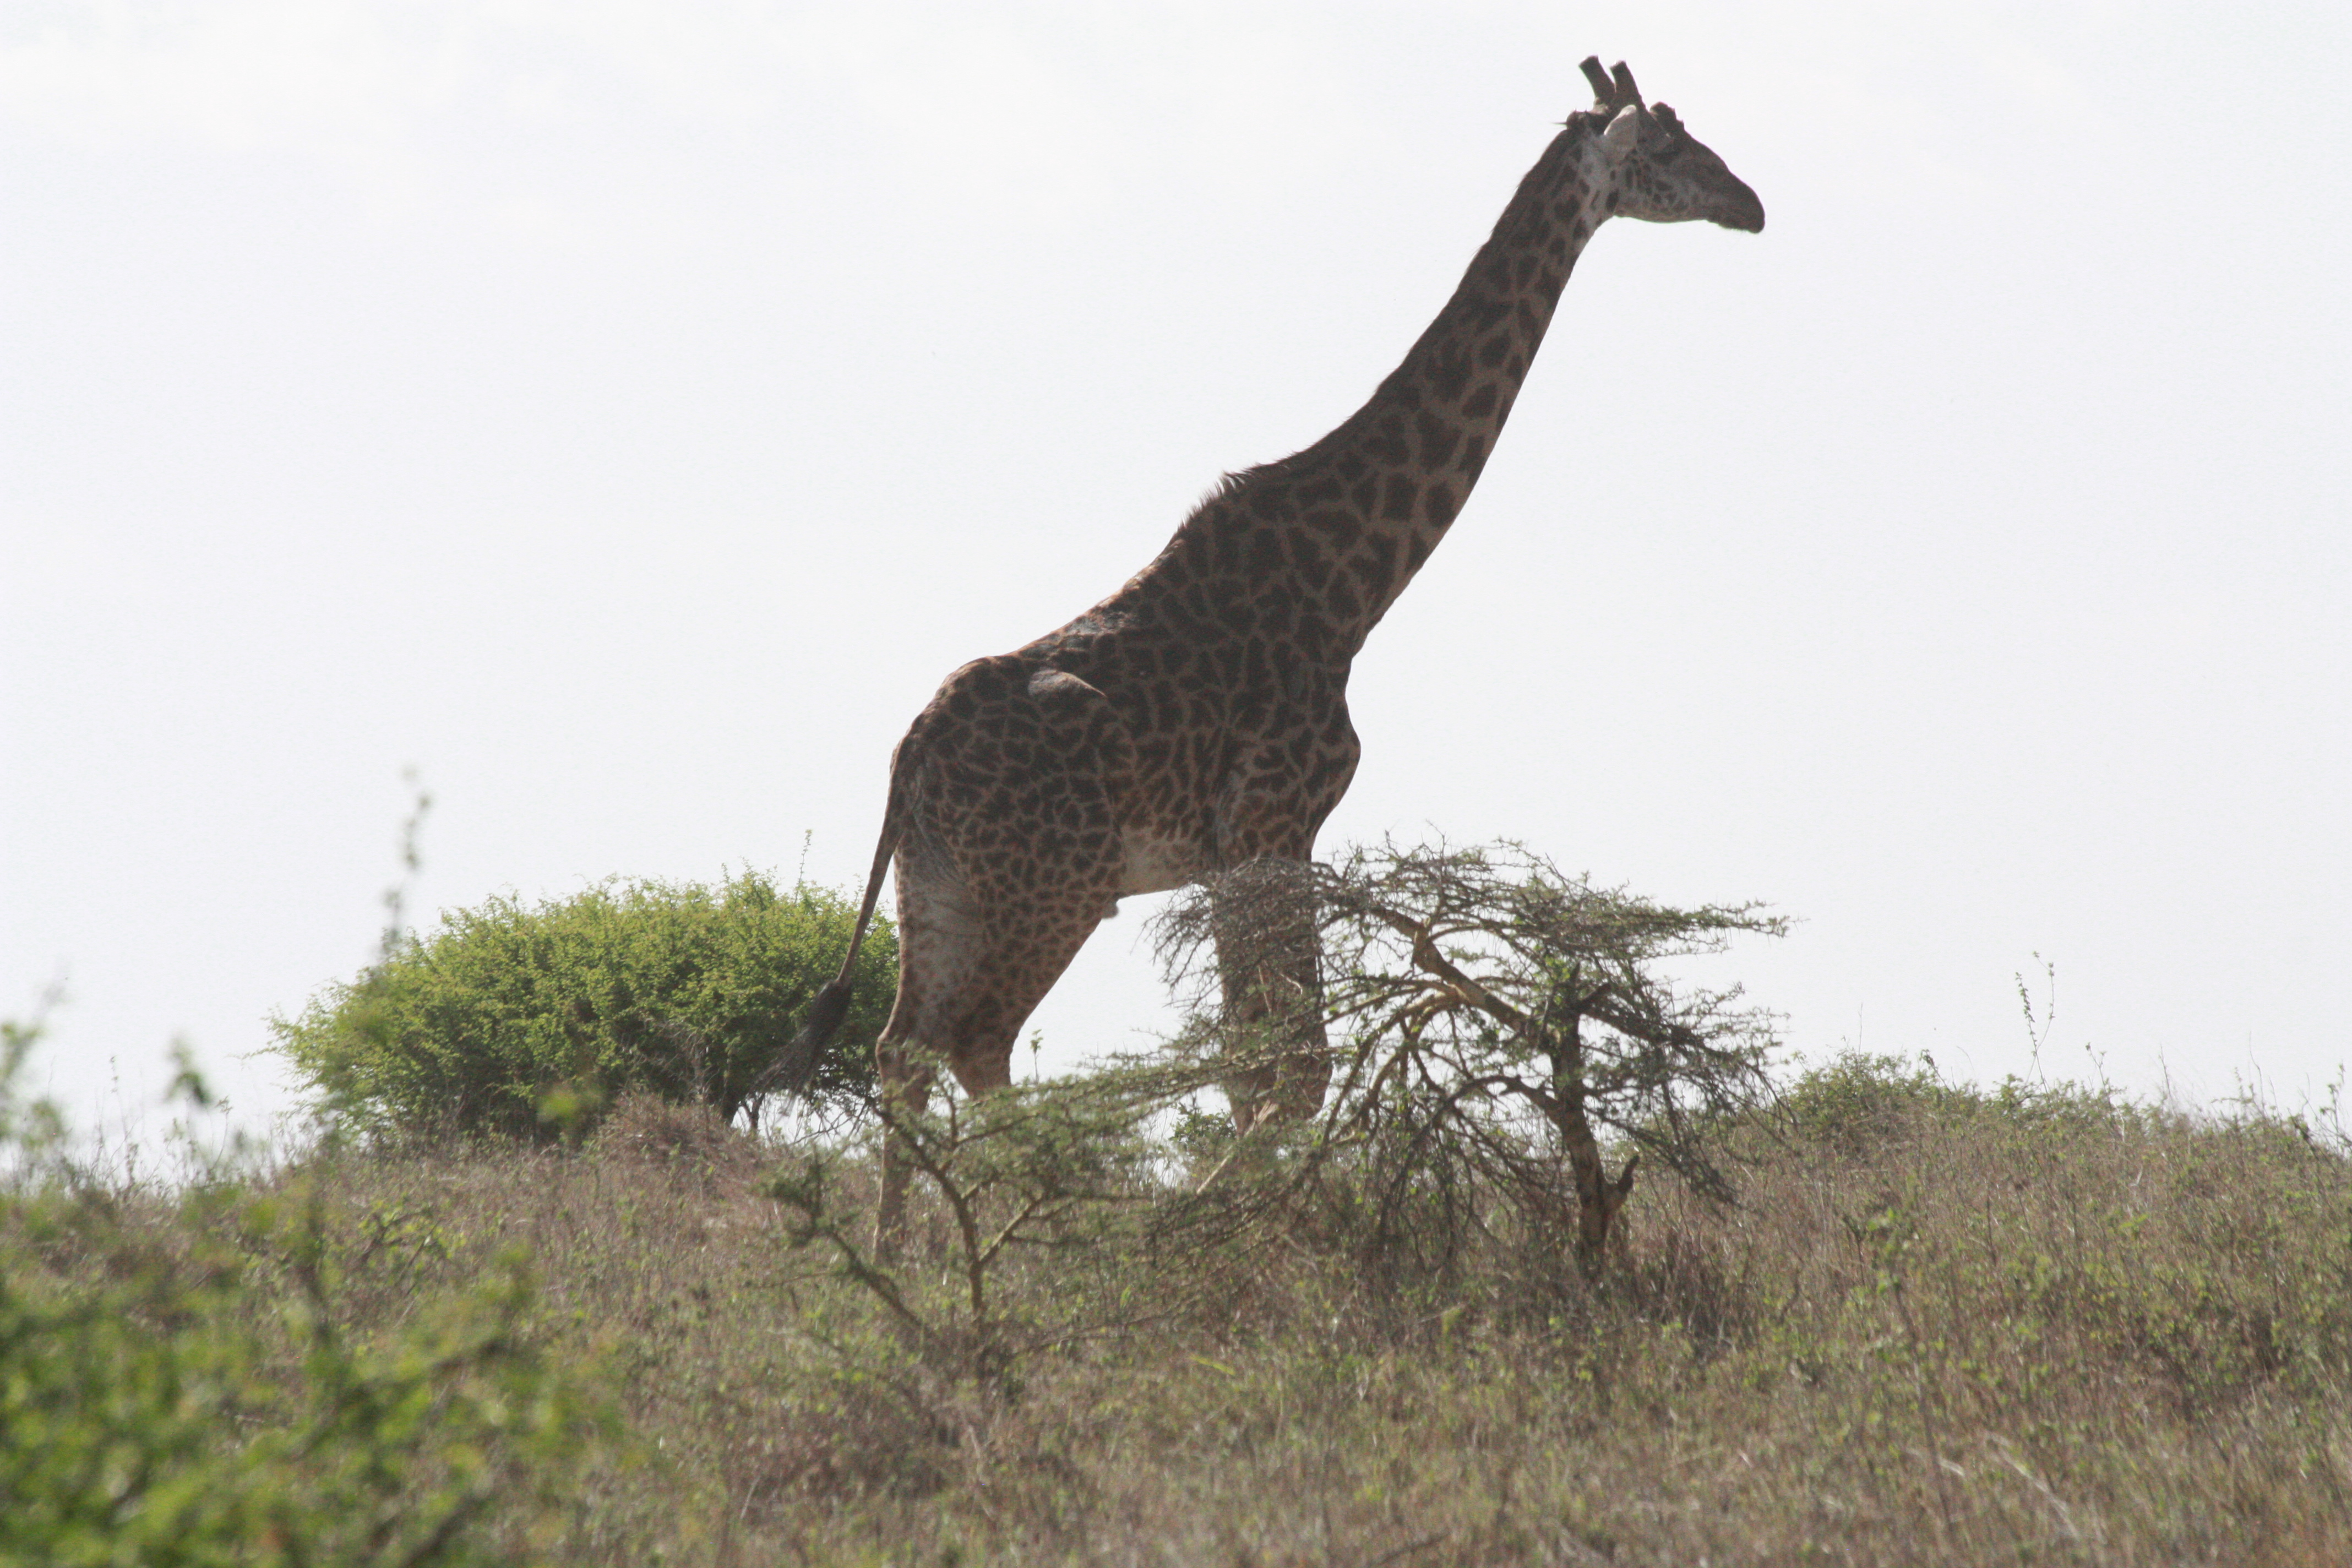
\includegraphics[width=0.16\textwidth]{resources/images/0c81eb06-0c4f-beba-cddb-858d59db523d.jpg} }}$ }}%
    \subfloat {{ $\vcenter{\hbox{ 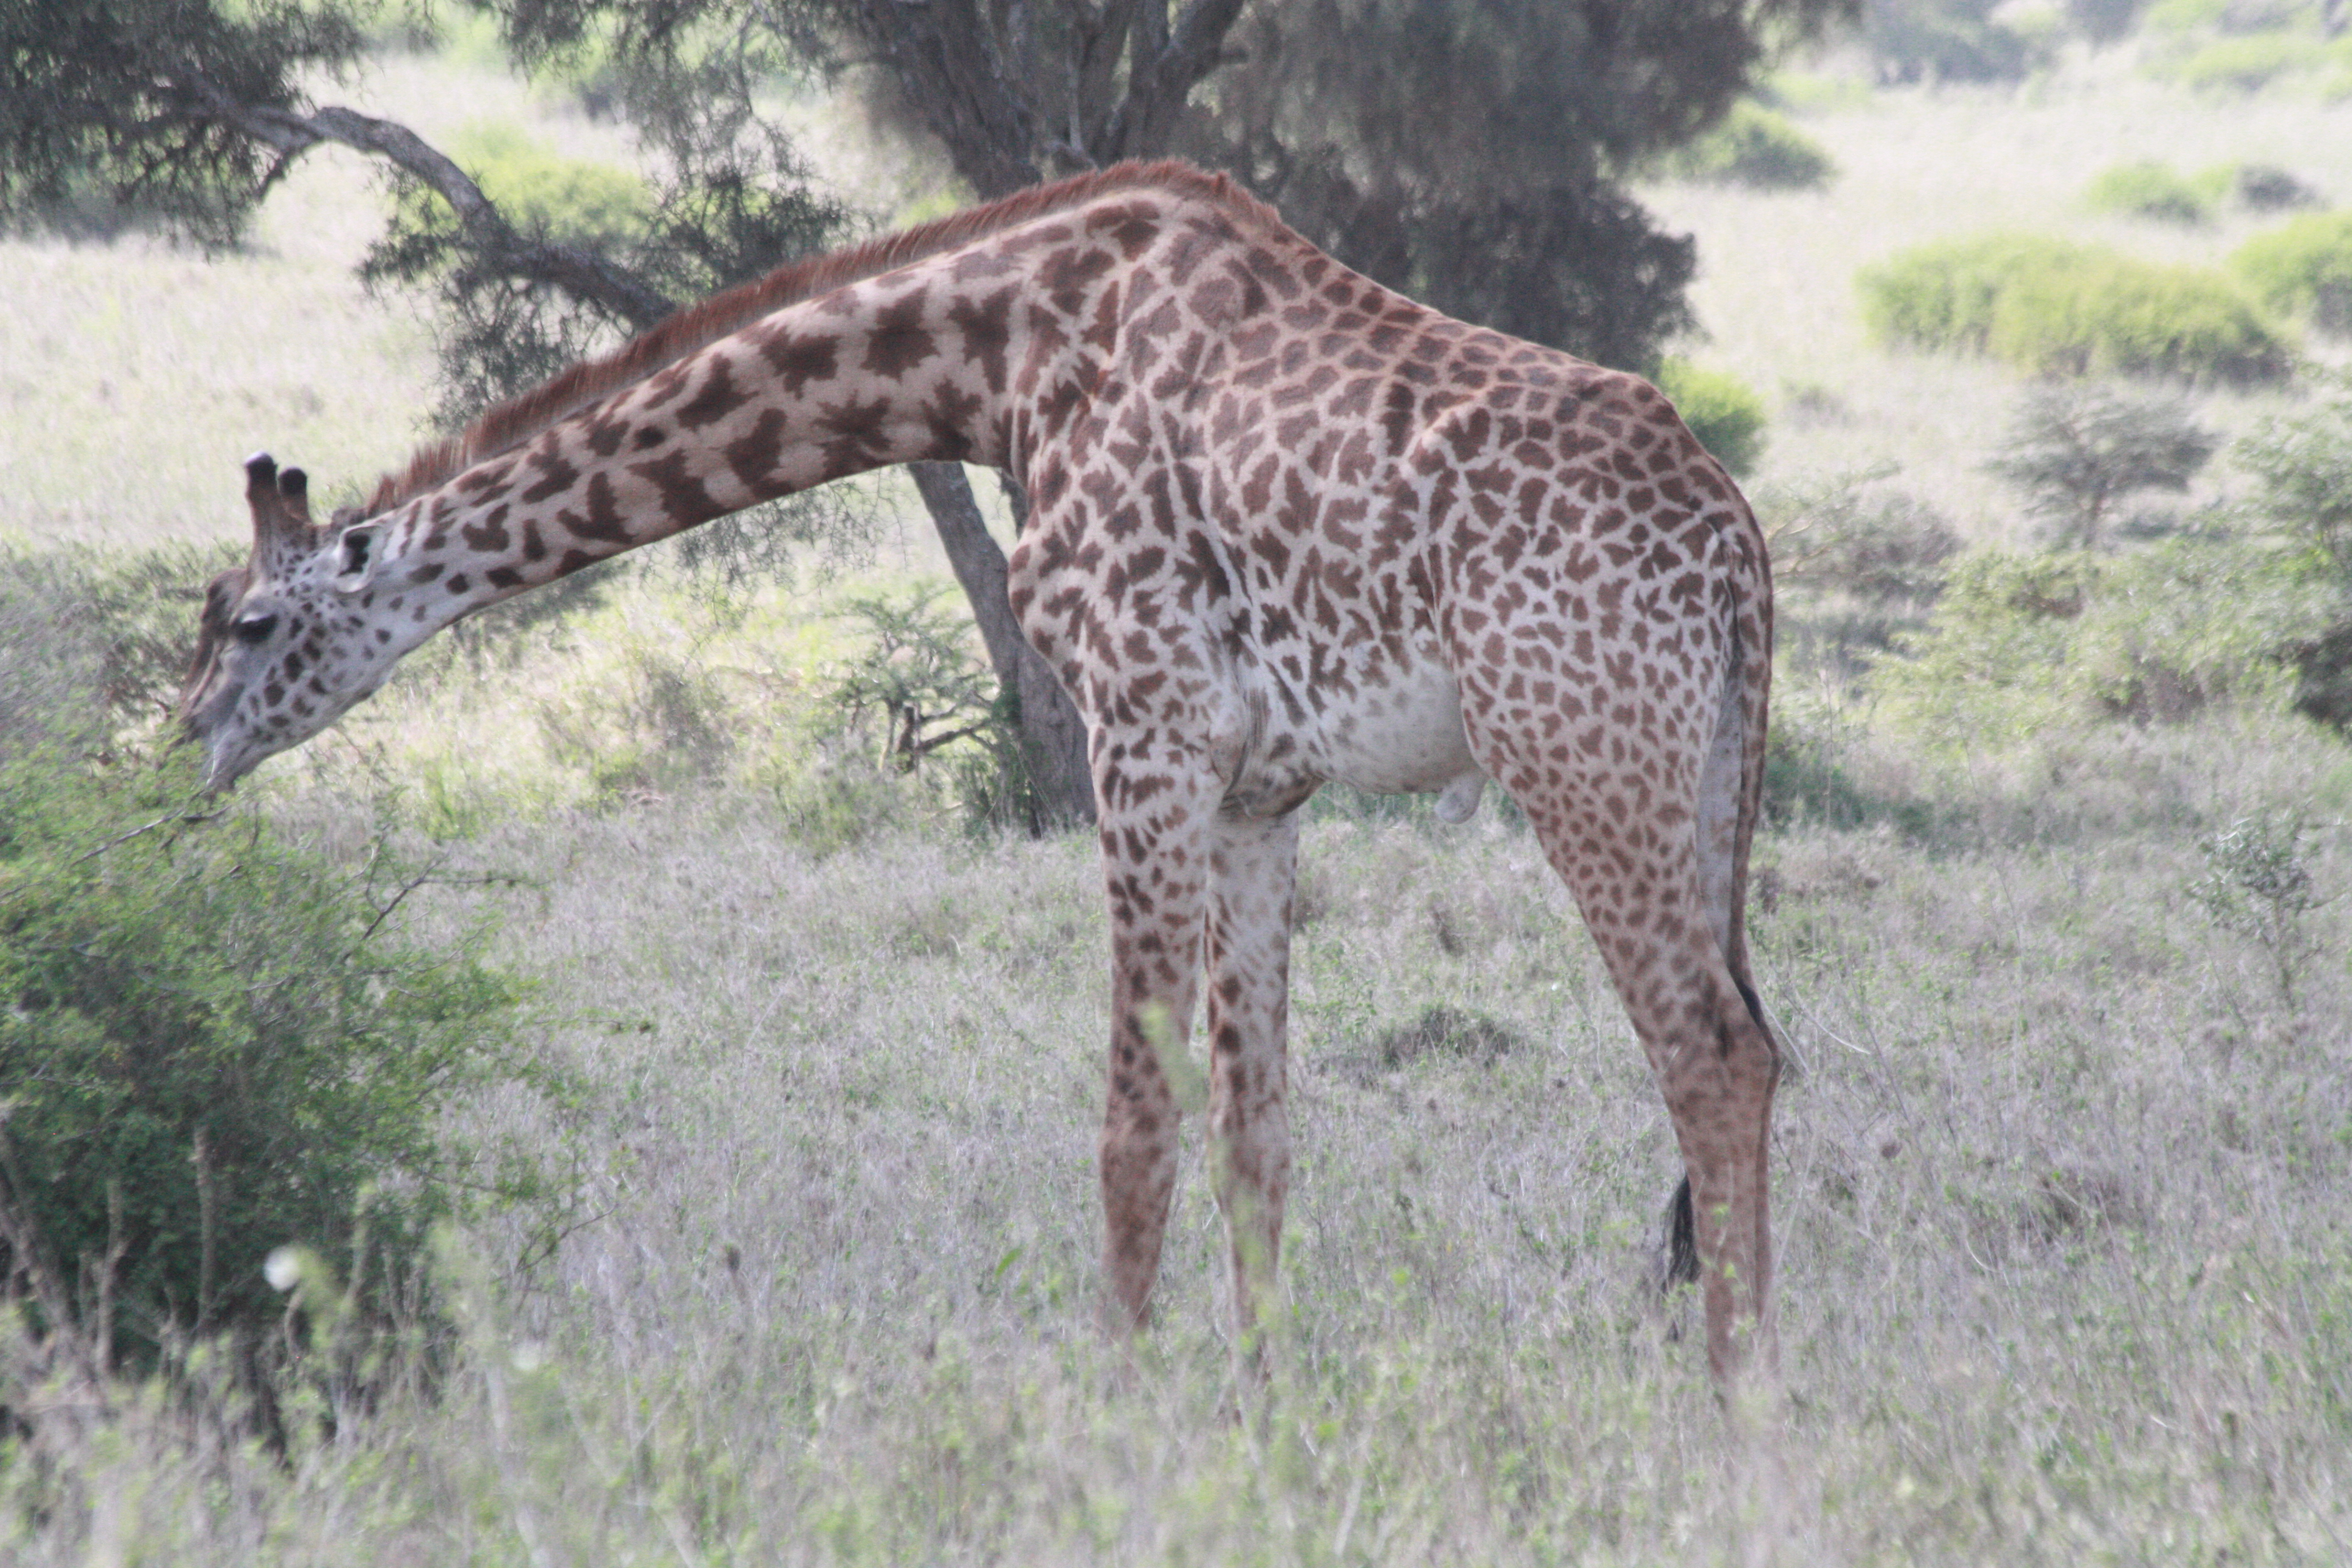
\includegraphics[width=0.16\textwidth]{resources/images/3d71a3d7-fef9-cfb4-0f28-c170338705f0.jpg} }}$ }}%
    \vspace{0.1cm}
    \subfloat {{ $\vcenter{\hbox{ 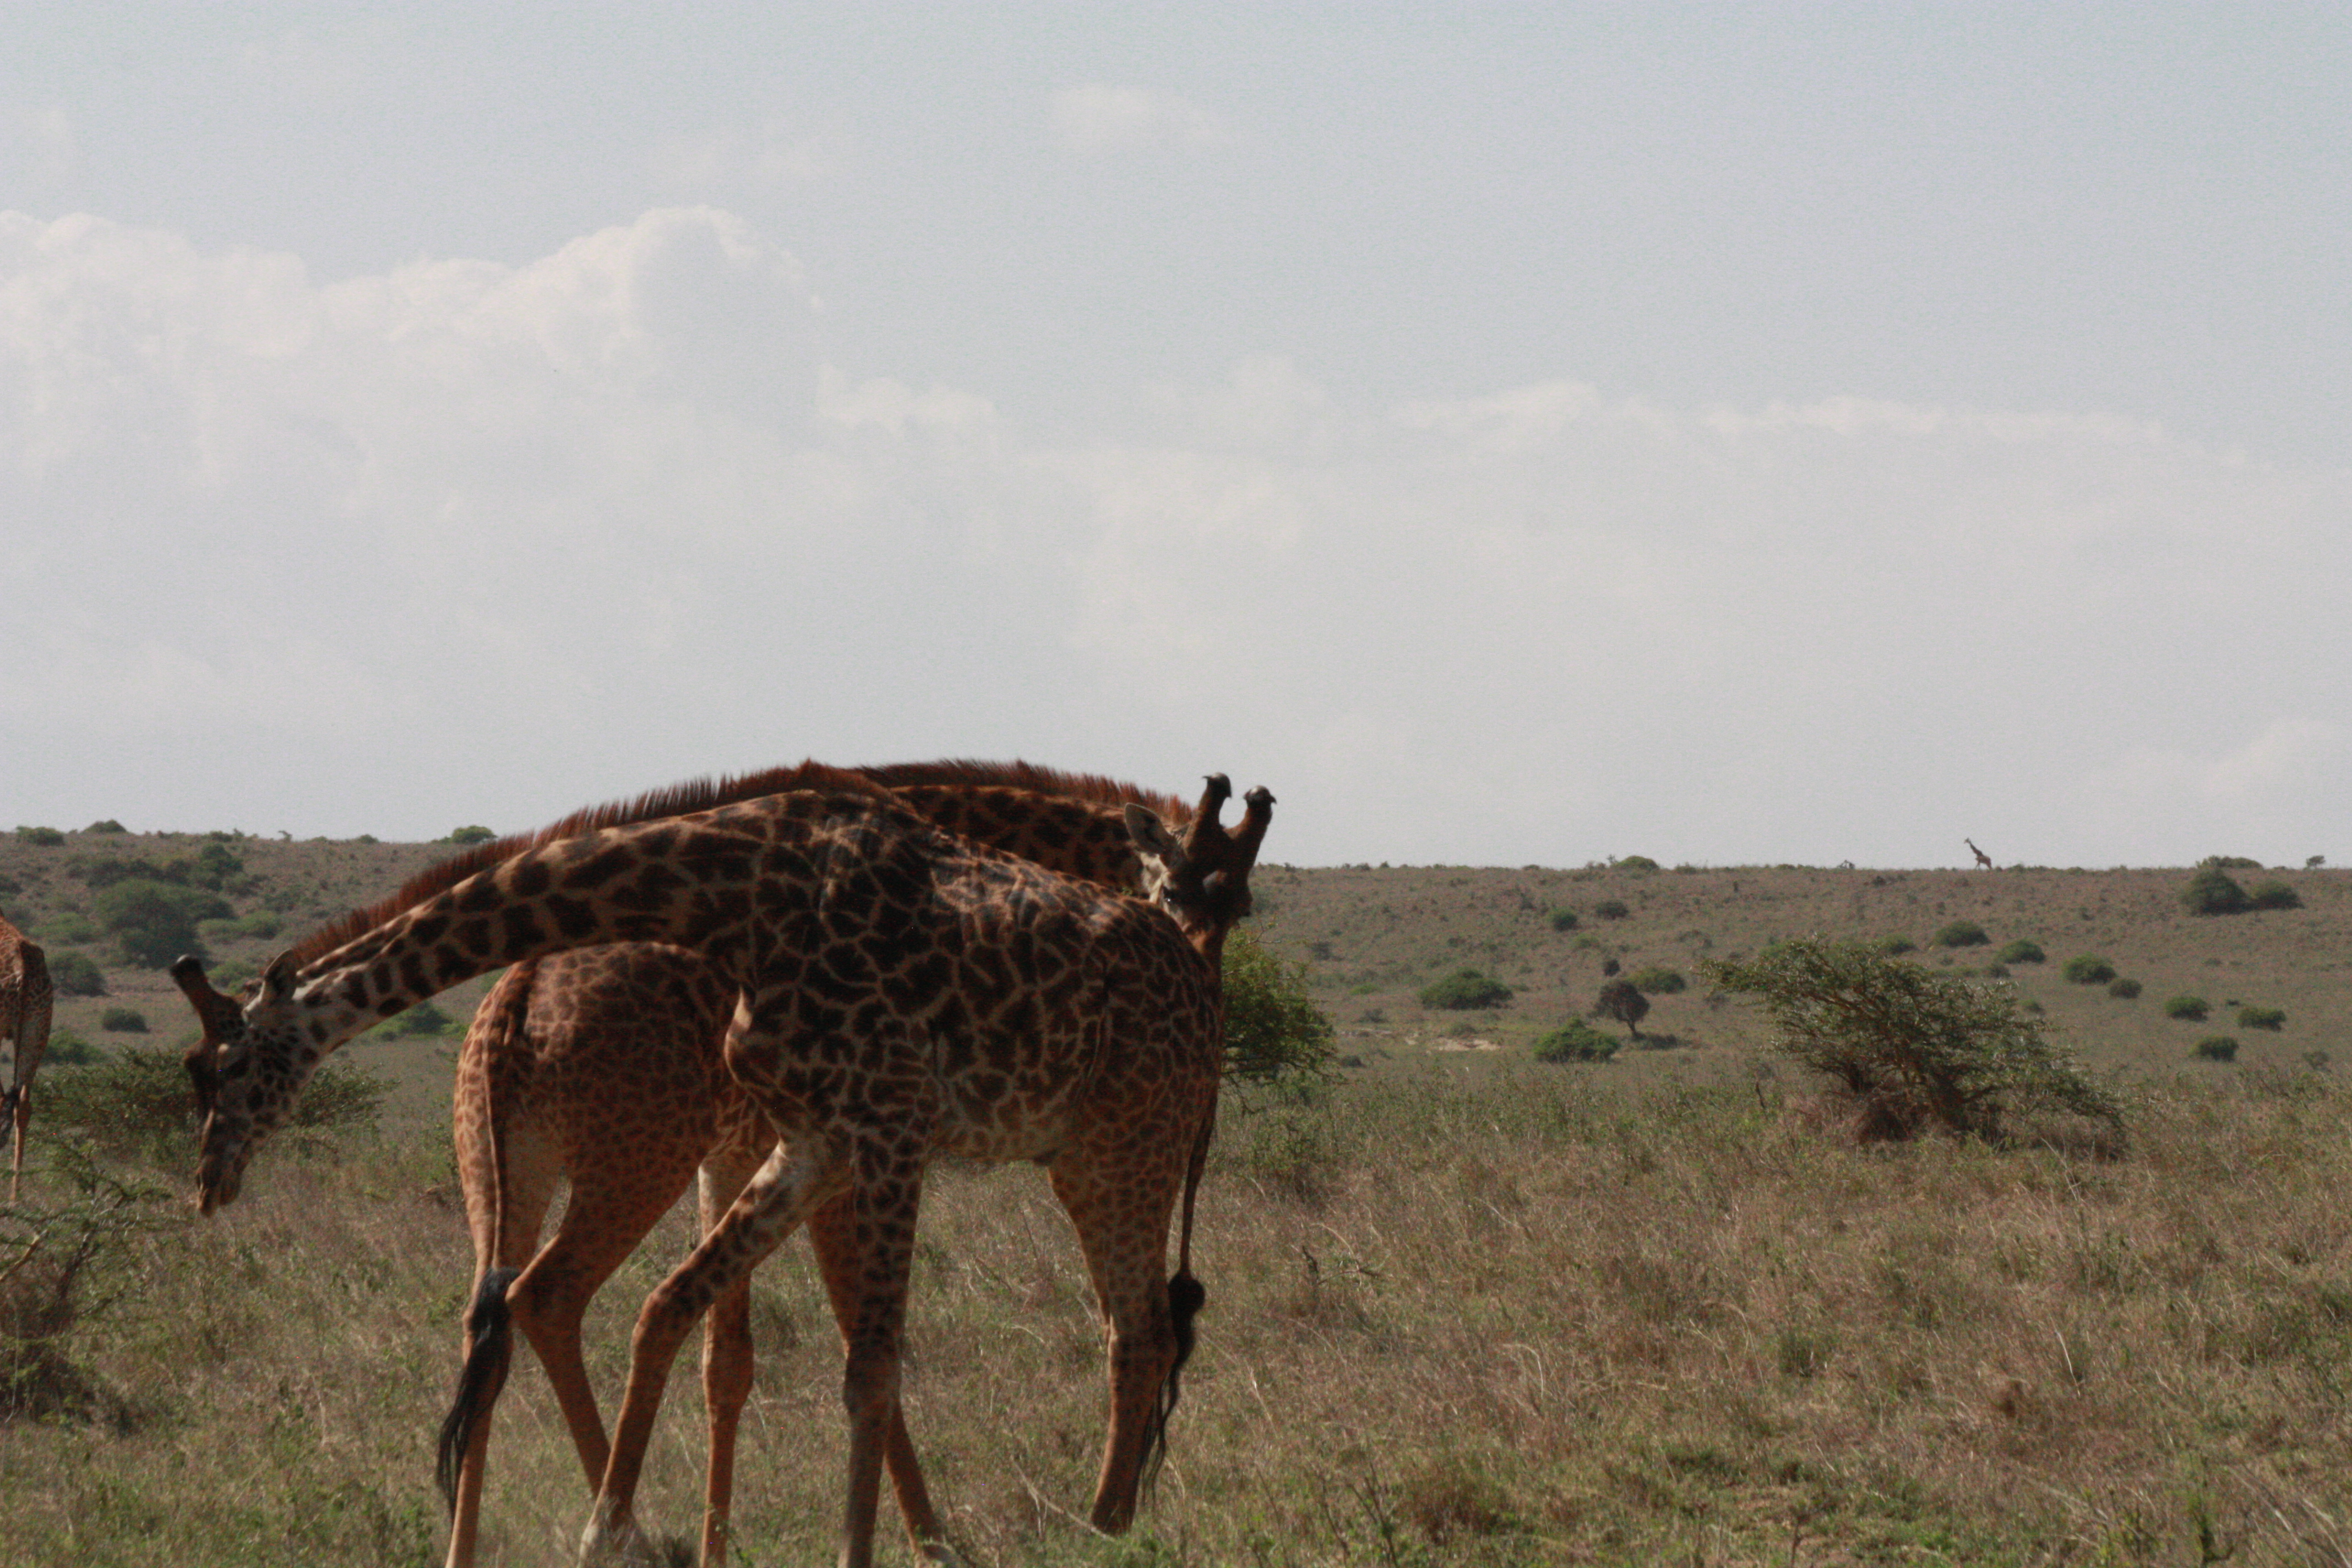
\includegraphics[width=0.16\textwidth]{resources/images/0c166bc9-7e21-6837-f09f-976a96f28f28.jpg} }}$ }}%
    \subfloat {{ $\vcenter{\hbox{ \includegraphics[width=0.16\textwidth]{resources/images/0c381b04-1651-4a1c-a24f-fe975a5f648d.jpg} }}$ }}%
    \subfloat {{ $\vcenter{\hbox{ \includegraphics[width=0.16\textwidth]{resources/images/0cf36e40-07f7-8003-adae-544b8416f4a0.jpg} }}$ }}%
    \subfloat {{ $\vcenter{\hbox{ \includegraphics[width=0.16\textwidth]{resources/images/0d0f8f63-3853-ae0f-409e-5ed351339045.jpg} }}$ }}%
    \subfloat {{ $\vcenter{\hbox{ 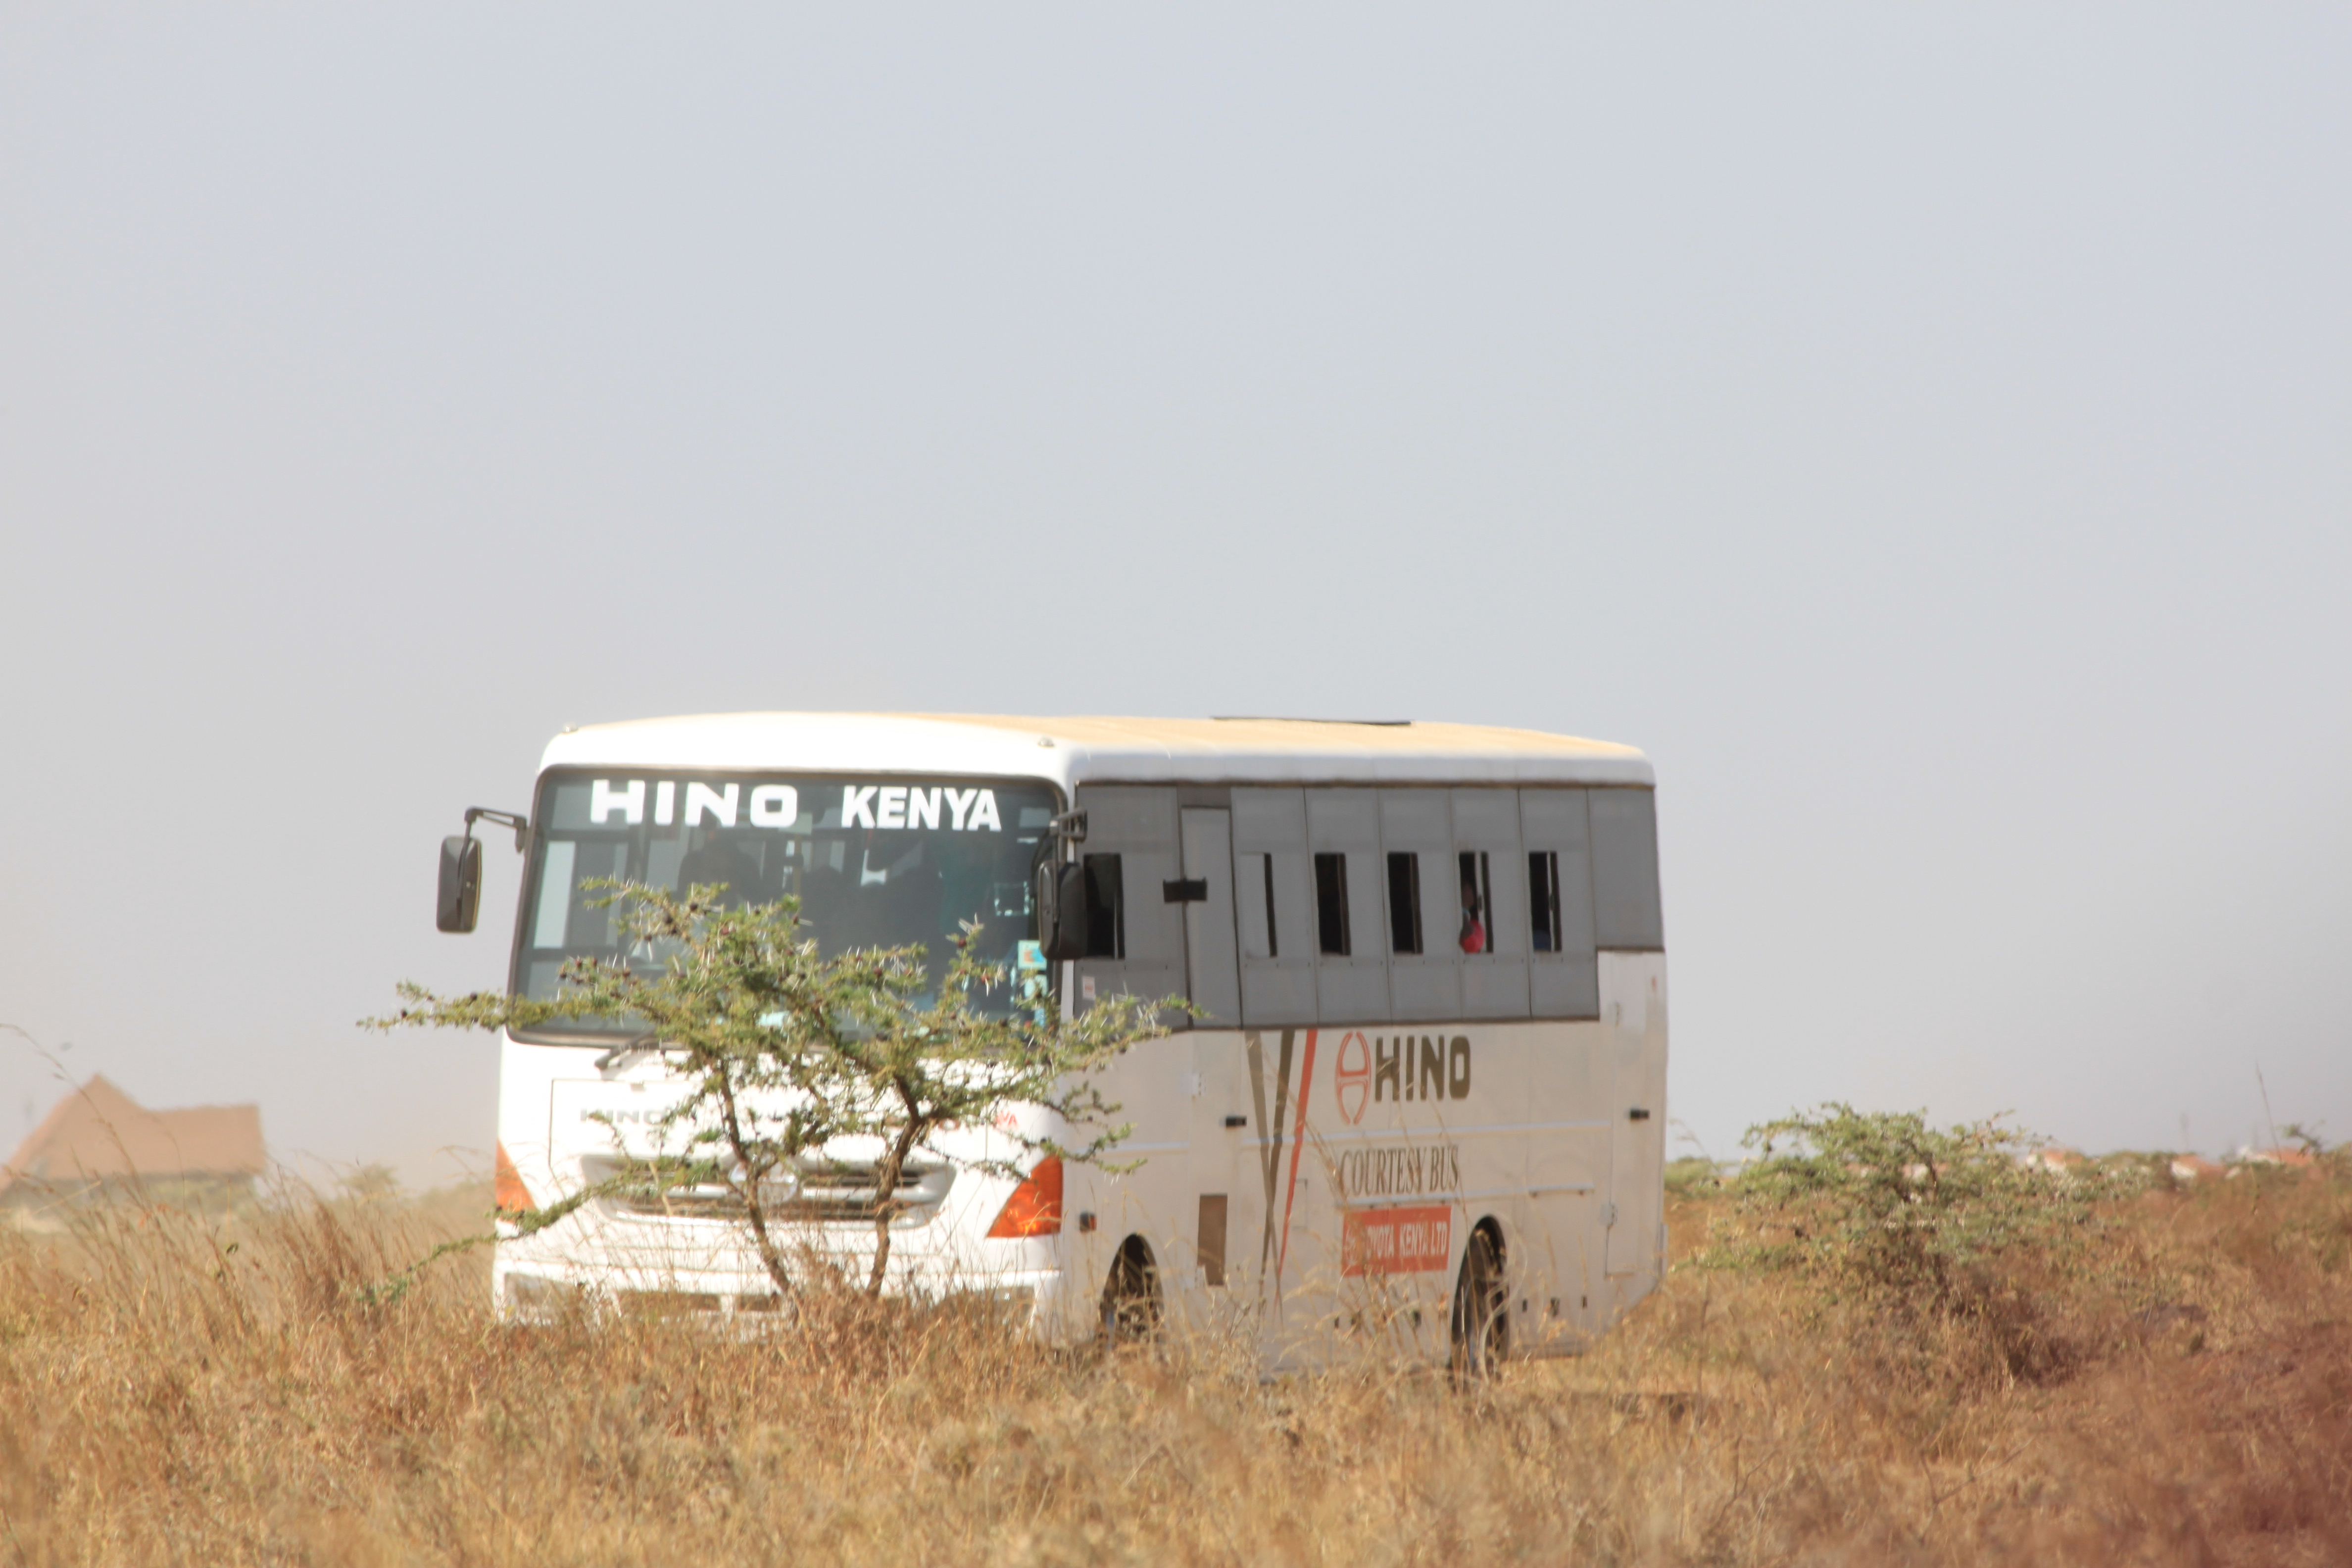
\includegraphics[width=0.16\textwidth]{resources/images/0e507f8d-b13c-b49d-fd19-f00d9570dbd7.jpg} }}$ }}%
    \vspace{0.1cm}
    \caption[Example Images Collected during \textit{The Great Zebra \& Giraffe Count}]{\textbf{Example Images Collected during \textit{The Great Zebra \& Giraffe Count}.}  A set of 10 example images collected from citizen scientists in the Nairobi National Park.  Images were collected from a variety of camera types, image formats, and across many hours throughout the day.  Most images contain sightings of zebra, giraffe, elephant, rhinocereous, cars, or birds from a wide range of focus, zoom, lighting conditions, and viewpoints of the animals.  There were also negative images collected having no animals in the forground, but instead had only road, cars, people, man-made structures, and planes, as shown in the bottom right image.  A total of 9,406 images were collected from all citizen scientists; a detailed breakdown of all images contributed can be found in Figure \ref{fig:contributions}.}
        \label{fig:images}
\end{figure*}

\section{Retrieval (Client)} \label{sec:retrieval}
Once the data collection was complete for a particular car, the participants were instructed to return to the registration site to contribute their images to the GZGC.

A participant's camera was required to have some form of removable memory card so that the images could be retrieved easily.  As such, mobile devices and camera phones were not recommended (but not explicitly excluded) for the sake of an efficient data collection workflow.  Fortunately for the GZGC, this was not considered much of a limitation considering most current mobile devices and camera phones do not have sufficient optical capabilities for capturing usable images.   Notably, the lack of a zooming lens and a limited optical sensor degrade the usefulness and quality of the images.  When no other camera was available to a participant, mobile devices and camera phones were permitted on the condition that the images could still be retrieved from a memory card or retrieval did not rely on dedicated or proprietary extraction software.  For the GZGC, we only had two contributors who took pictures using a mobile device.  The images contributed by these citizen scientists were not of optimal quality and IBEIS had trouble identifying correct matches due to lens artifacts and the photographed animals being too small in the image.

For other data collection events, a mobile data collection device might be tolerable (or even preferred) and a more sophisticated workflow or mobile application (app) could be created to facilitate offloading the image data from the device.  An app could be downloaded to the phone and used to collect and annotate using a light-weight, touch-based user interface.  The app could also implement a communication protocol that would allow sending the collected images directly to a central server for processing, without the need to download the images to a client machine.

Using the registration card, the participant's camera memory card, and the car's GPS dongle, all of the information required for processing could be gathered:

\begin{enumerate}
    \item Using the participant's physical registration card, the participant's identification code and the file name (or sequence number) for $Image_0$ could be recovered.
    \item Images were copied, in order of the EXIF timestamp provided by the camera, from the memory card starting at $Image_0$.  All images were copied locally to the import client laptop and a copy was saved onto an attached backup external hard-drive.
    \item The registration card also provided when $Image_0$ was taken in Nairobi local time.  Therefore, assuming the camera was properly keeping time and the EXIF timestamps were self-consistent, all images taken by that camera could be synchronized to Nairobi local time.
    \item The car's GPS dongle provided the location of the car (and therefore the participant and their personal camera) with a series of UTC-timestamped GPS records.  The time-synchronized images were synchronized with UTC/GMT using the timezone offset for Nairobi (UTC+3) and the GPS location of each image was retrieved by performing a lookup search in the GPS records.  When the exact time (accuracy of a second) was not recorded, we took the last known position of the GPS dongle that was closest in time to the query time.  Missing times could be a result of a dropped GPS signal acquisition, poor signal strength, the dongle losing battery power, or the dongle being accidentally turned off.  Fortunately, none of GPS tracks recorded for the GZGC had large unintentional time gaps and almost all query times could be found absolutely (give or take a second).  This last-known scheme could easily be replaced with interpolation between the two closest-in-time recorded GPS locations.  We opted to not perform interpolation in order to prevent images from being localized off-road or outside the boundary confines of the park considering that the park's roads and boundary form a concave mesh.
    \item The car's assigned data collection zone within the park.
\end{enumerate}

\begin{figure}[t]%
%\begin{figure}[!htb]%
    \centering
    \subfloat {{ $\vcenter{\hbox{ \includegraphics[width=0.90\textwidth]{resources/client-image.png} }}$ }}%
        \caption[The Retrieval (Client) Image Submission Interface]{\textbf{The Retrieval (Client) Image Submission Interface.}  The client interface was used to submit a subset of a citizen scientist's images to the IBEIS server for processing.  Images were copied from the memory card and 12 images (10 randomly selected plus the first and last) were displayed on the right.  The information for the contributor was added to the left-hand side and could be inputted (in parallel) as images were being copied locally.}
        \label{fig:client-images}
\end{figure}

\begin{figure}[t]%
%\begin{figure}[!htb]%
    \centering
    \subfloat {{ $\vcenter{\hbox{ \includegraphics[width=0.90\textwidth]{resources/client-gps-fixed.png} }}$ }}%
        \caption[The Retrieval (Client) GPS Submission Interface]{\textbf{The Retrieval (Client) GPS Submission Interface.}  The client interface was also used to extract and submit the GPS dongle track information associated with a particular car.  As with images, GPS tracks were copied from the dongle in parallel as contributor information was added to the left.  The track of the dongle was displayed on the map to the right before being submitted to the server.  The GPS information was recorded for a \textit{car} and was inherited by all participants in that car.}
        \label{fig:client-gps}
\end{figure}

When the participant's registration card was lost or unreadable, the participant's images were manually searched (starting from the most recent image taken and working backwards in time) for $Image_0$.  Once $Image_0$ was found, the participant's identification code and local time of registration could be extracted.  Searching for $Image_0$ could be done automatically using computer vision algorithms looking for the card's visually distinctive features, but unfortunately this was not completed in time to be used for the GZGC.

Each participant returned from collection with a camera card full of digital images.  See Figure \ref{fig:contributions} for the breakdown of how many images were contributed by each participant.  The semi-automatic processing by IBEIS was too computationally involved to process all of the contributor's images on-site and on-demand.  Instead, we opted to process only a small subset of $X$ images for each participant to produce printout results (see Section \ref{sec:feedback}) -- for the GZGC, we set $X=10$, meaning we needed to only process 10 images on-site for each participant.  All images were saved for processing until the GZGC was finished and computational constraints were no longer an limiting concern (see Chapter \ref{sec:analysis}).  Overall, this was not considered a limitation because it eliminated complexity in the collection procedure and is justified because only a handful of images were required to generate the printout.  Without this reduction, the GZGC would not have been nearly as interactive and engaging nor would it have been as compelling for citizen scientists to re-participate in a future data collection event due to delays or inaccuracies.

The import client, shown in Figures \ref{fig:client-images} and \ref{fig:client-gps}, was responsible for copying the images from the memory card and also deciding which subset of images was to be submitted to the server for processing.  In parallel, and as the images were being copied from the memory card (an operation that took several minutes), the import client randomly and automatically selected images for a pre-trained, IBEIS volunteer submitter to review.  If any of the selected candidates did not have a zebra (or giraffe) or did not otherwise satisfy the data collection protocol, a new candidate could be randomly selected by simply clicking on the image.  Once the set of $X$ candidate images was finalized, the opportunity was given to the reviewer to add additional metadata to the image, such as the dominant species (zebra or giraffe) in the photograph.  For the GZGC, IBEIS required the dominant species to be annotated to help facilitate detection.  Future versions of IBEIS will overcome this requirement by employing the techniques described in Chapter \ref{sec:verification}.  The system also had the functionality to accept fewer than $X$ images, in the event that a photographer did not have enough quality animal sightings.  The final selected subset of $X$ images for the participant was sent to the central server for processing, which at that point should have only contained quality, left-side images of zebras or giraffes.  % The processing step was required to ultimately generate immediate feedback to give to each volunteer photographer.

\begin{figure}[t]%
%\begin{figure}[!htb]%
    \centering
    \subfloat {{ $\vcenter{\hbox{ \includegraphics[width=0.90\textwidth]{resources/contributions.png} }}$ }}%
        \caption[The Number of Images Contributed by All Citizen Scientists]{\textbf{The Number of Images Contributed by All Citizen Scientists.}  The number of images contributed by each citizen scientists ranged wildly from a handful to over 450.  The bottom axis displays the car number designation, the bar color indicates the car's assigned color, and the letter above the bar specifies the individual contributor in that car.  The height of the bar gives the number of images contributed by that participant.  Red cars were assigned on the first day of the GZGC, whereas the white cars were assigned on the second day.  The color blue was given to cars that skipped or failed to complete the registration process, but had images to contribute; due to the lack of registration, the blue colored cars were missing GPS information.  The purple color was reserved for dignitaries and IBEIS team members.}
        \label{fig:contributions}
\end{figure}

\section{Processing (Server)}
The IBEIS central server was responsible for processing a volunteer's submitted images sent from any import client.  The IBEIS computer vision system took images (along with their associated metadata) as input, processed the images by finding any zebras (or giraffes) in the image, searched a database for each sighting to find the closest matching zebras (or giraffes), and outputted the highest scoring match (along with the match's metadata).  Figure \ref{fig:detections} shows example automatic detections (orange bounding boxes) found by IBEIS around different sightings of animals.  Note that the animal detector, which was trained to detect zebras and giraffes, did not place a box around the rhinoceros.  Therefore, the detector also functioned as a filter to prevent sightings of other animals or images with no animals from being processed.  The detector was also fairly responsive to blurring and image noise, which also acted as an implicit, built-in quality filter.  Finally, the detector had to function across many scales and viewpoints of animals.

To perform identification on a citizen scientist's sightings, IBEIS needed the GPS information from that participant's car and their images.  To prevent from having to submit duplicate GPS information repeatedly for each participant in a car, we enabled a caching system; the caching system either saved images for a participant until their car's GPS was submitted or saved a car's GPS information for the images of any subsequent participant in that car.  This caching allowed an asynchronous and order-agnostic submission workflow and significantly reduced the complexity of the data collection for the GZGC.  This feature cannot be simply overlooked; it was a critical component to the smooth execution of the GZGC.  Without it, the client machines would have been forced to adhere to a rigid and brittle submission procedure.  For example, requiring GPS to be submitted for each and every participant, requiring GPS be submitted before any participants in that car, while requiring participants to submit in alphabetical order based on their registration letters would not only have been a logistical headache but would have damaged the efficiency and fluidity of the data collection.  The asynchronous, distributed, and caching submission protocol circumvented all of these issues, which allowed images to be submitted in any order, by participants in any order, and independent of their respective GPS information.  For any cached submissions, once the required image and GPS information had been acquired by the server, it immediately launched IBEIS processing on the cached data and triggered a results review interface.  This sometimes resulted in a burst of results needing review.  They were reviewed one-at-a-time to generate the feedback printouts.

\subsection{Feedback Generation} \label{sec:feedback}

\begin{figure*}[t]%
    \centering
    \subfloat {{ $\vcenter{\hbox{ \includegraphics[width=0.16\textwidth]{resources/detections/3e4aa7cb-822a-c360-4068-994c1bc30b0e_500_thumb.jpg} }}$ }}%
    \subfloat {{ $\vcenter{\hbox{ \includegraphics[width=0.16\textwidth]{resources/detections/3c691d2d-c93f-2cf9-1cbe-1326902bedce_500_thumb.jpg} }}$ }}%
    \subfloat {{ $\vcenter{\hbox{ \includegraphics[width=0.16\textwidth]{resources/detections/03cb09e0-600a-f0cd-8af5-aea64db78050_500_thumb.jpg} }}$ }}%
    \subfloat {{ $\vcenter{\hbox{ \includegraphics[width=0.16\textwidth]{resources/detections/3cc3521d-7fee-21a3-3b84-427537f6102a_500_thumb.jpg} }}$ }}%
    \subfloat {{ $\vcenter{\hbox{ \includegraphics[width=0.16\textwidth]{resources/detections/3f15c6f9-5b38-0243-fca8-19c105b1b17f_500_thumb.jpg} }}$ }}%
    \vspace{0.1cm}
    \subfloat {{ $\vcenter{\hbox{ \includegraphics[width=0.16\textwidth]{resources/detections/3d8bbc50-fbec-2e80-4993-04542aeb5ef6_500_thumb.jpg} }}$ }}%
    \subfloat {{ $\vcenter{\hbox{ \includegraphics[width=0.16\textwidth]{resources/detections/3d355406-91a4-00b5-955a-e714eb876796_500_thumb.jpg} }}$ }}%
    \subfloat {{ $\vcenter{\hbox{ \includegraphics[width=0.16\textwidth]{resources/detections/3bc474d4-16df-ce29-ca9a-9d43775e62d2_500_thumb.jpg} }}$ }}%
    \subfloat {{ $\vcenter{\hbox{ \includegraphics[width=0.16\textwidth]{resources/detections/3ee3167c-9c96-e627-a098-2ee8dea8f303_500_thumb.jpg} }}$ }}%
    \subfloat {{ $\vcenter{\hbox{ \includegraphics[width=0.16\textwidth]{resources/detections/3ca2a9c0-4f0e-2099-12b7-2bba21e69834_500_thumb.jpg} }}$ }}%
    \caption[Example IBEIS Automatic Detections]{\textbf{Example IBEIS Automatic Detections.}  Images taken by citizen scientists during \textit{The Great Zebra \& Giraffe Count} were automatically detected using computer vision algorithms to find sightings of animals.  Animal detections were performed across different species with the goal of locating animals at any arbirary location or scale in the image.}
        \label{fig:detections}
\end{figure*}

Volunteer photographers participating in the GZGC were incredibly enthusiastic about their contributions to the population count.  All were rewarded for their contribution with a printout that mapped their car's route using the GPS data, the three images selected for the printout, the three images' recognition state, and the locations of other sightings for those three individuals on the map.  Involving the citizen scientists in conducting research not only generates an appreciation for the animal populations in the NNP (which are common and largely ignored by Nairobi citizens), but can also be an attraction for fee-paying park visitors who would not have attended otherwise.

We wanted to provide immediate feedback showing information about the identities of the animals each contributor photographed.  Since the majority of contributors took over 100 images, and considering that processing took around 10 seconds per image, we could not give complete feedback on all images.  This limitation was not only due to computational resource limitations, but also due to the fact that the IBEIS results for all images had to be manually reviewed to confirm their accuracy.  Instead, we decided to give feedback on the processing results for just three of their images.  Since the goal of the GZGC was to ultimately count the unique individuals, we reported feedback on whether each individual had ever been seen before and, if so, where it had been previously sighted in the NNP.  In order to provide this level of feedback to the first contributors, it meant we needed to build an initial IBEIS recognition database.  The initial database was compiled using images taken over 9 days prior to the GZGC and consisted of 2,188 images sampled throughout the NNP.
It should be noted that 10 images were sent for processing for each contributor knowing that only three of their images were to be selected for the printout.  The reason for this was to virtually guarantee at least one resighted animal and to eliminate the need to resubmit images for a participant if problems arose (e.g.\ detection failures, poor quality images, no matching animals in the initial database, or any other unforeseen issue).  The triple redundancy also allowed the reviewer to select the three best or most engaging matches.

As seen in Figure \ref{fig:client-printout}, each of the three images on the printout was labelled as either a new animal or a matched animal.  When the sighting was a new zebra (i.e.\ not seen in the initial database), the citizen scientist was rewarded with the knowledge of finding a never-before-seen individual and incrementing the total number of zebras known to be in the NNP.  The information contributed by the citizen scientist about this new zebra (image, location, time, etc.)\ established a permanent record for that individual in the database and was queried against for future participants.  In the event of the sighting being a known zebra (i.e.\ matched in the initial database), the citizen scientist was rewarded with the knowledge of adding relevant information to that individual's record.  The information contributed by the citizen scientist about this resighted zebra gives conservationists information about the movement and migratory patterns of that individual.

\begin{figure}[t]%
%\begin{figure}[!htb]%
    \centering
    \subfloat {{ $\vcenter{\hbox{ \includegraphics[width=0.90\textwidth]{resources/review_interface.png} }}$ }}%
        \caption[The IBEIS Results Review and Feedback Generation Interface]{\textbf{The IBEIS Results Review and Feedback Generation Interface.}  The IBEIS results (left) were displayed to a reviewer to verify if found matches were correct.  Correct matches were selected and automatically placed into the printout template (right) for the contributor.  Once the selection of three images was finalized, the reviewer sent the template for PDF generation and the resulting file was printed.  The GZGC did not have Internet access, but the digital PDF copy of the printout was emailed to the citizen scientist upon request.}
        \label{fig:client-printout}
\end{figure}

During the GZGC, we had the honor of having the U.S. Ambassador to Kenya Robert F. Godec and staff participate in the collection of images in the NNP.  Figure \ref{fig:printout-godec} in the Appendix shows his printout and the three results from his data collection.

In summary, the data collection event was successful in its two primary goals: to copy images from the camera memory cards for future processing (described in the next Chapter) and to provide an engaging and rewarding experience for the volunteer citizen scientists.  The design of the GZGC and its software interfaces was as much about marketing outreach and establishing public relations as it was about the easy and distributed collection of images for a population study.  It was vitally important to provide a positive experience for all participants in order to encourage word-of-mouth promotion and to hopefully ensure future re-participation.  The strength of the GZGC and any future events depends crucially on the time and efforts of volunteer photographers.  % We would like to thank all of the citizen scientists that participated in the GZGC for their contributions

Other than the volunteer citizen scientists contributing images, the IBEIS team also consisted of volunteer Nairobi students who were trained to help guide participants through the registration and submission process.  These IBEIS volunteers were the front line and face of the GZGC and were instrumental in maintaining a smooth and functional workflow during peak times.  Insufficient or incorrect information during the training of the IBEIS volunteers could have easily led to either registration inconsistencies -- and thus synchronization failures -- or submission workflow inefficiencies.  They key to producing an effective team of volunteers is providing a focused and easy-to-use software interface for the submission and processing review.

Finally, it should be noted that most of the effort and care in designing the collection workflow and software interfaces was focused on resolving the time and GPS synchronization and maximize camera compatibility.  The effectiveness of the entire GZGC hinged on the IBEIS team's ability to reconstruct the precise time and location where a sighting of an animal actually happened.  Future data collection events should seriously consider providing camera equipment with in-camera GPS to the volunteer citizen scientists, which eliminates some of the complexity from the procedure above and almost all of the synchronization issues.  For bigger data collection events, this procedure could also be easily scaled up to incorporate additional import client machines and additional processing power by adding more IBEIS-powered processing servers.  The delays and processing times during the GZGC were tolerable during heavy load as the entire process was structured around an efficient import, submit, process, review, print pipeline, where each stage could be distributed and completed in parallel.
